\documentclass[a4paper,12pt]{article}
\usepackage[utf8]{inputenc}
\usepackage{mathtools}

% Allow the change of line spacing
\usepackage{setspace}
\usepackage{tabularx}
\usepackage{graphicx}
\usepackage[usenames,dvipsnames,table]{xcolor}

%\usepackage{hyperref}
%\usepackage{breakurl}

%opening
%\title{Trainmining}
%\author{Grupo de Sistemas Inteligentes \\ Universidad Politécnica de Madrid}


\begin{document}
\newcommand\litem[1]{\item{\bfseries #1 }}
\renewcommand{\arraystretch}{1.5} %Makes tables less crammed

\newcommand\headcell[1]{%
  \multicolumn{1}{c|}{\cellcolor{MidnightBlue}\bfseries\sffamily\textcolor{white}{#1}}
}

%\renewcommand{\abstractname}{Executive Summary}
%\begin{abstract}
%
%\end{abstract}

% Set line spacing to 1.5
\onehalfspacing

% Begin a new titlepage. Tit	lepages have special settings like the absence of page numbers.
\begin{titlepage}
\sffamily
% Set the text of the page to right-aligned until \end{flushright}
\begin{flushright}

% Set the space between right page border and text to 2.5cm
\rightskip=-1cm

% Show an image at this position

\includegraphics[scale=1]{./img/logoGSI.png} 
%\includegraphics[bb=0 0 204 110]{web40logo.png}

% Skip a little space
\bigskip
\bigskip
\bigskip



% Create a title for the document and write it in bold font
\LARGE{\textbf{Deliverable 3. Knowledge Discovery results.}}
% Again, do a line break
\linebreak
% Create a subtitle
\large{Evaluation and interpretation.}

% Skip some space
%\bigskip
%\bigskip
%\bigskip
%\bigskip
\bigskip

% Write in very large letters
\LARGE{Grupo de Sistemas Inteligentes}
\linebreak
\large{Departamento de Ingeniería de Sistemas Telemáticos}
% Do a line break right after the \LARGE{...} text
\linebreak
% Write in large letters
\large{Universidad Politécnica de Madrid.}

% Skip some space
\bigskip
\bigskip
\bigskip
\bigskip
\bigskip
\bigskip

\large{Project Report}

% Skip some space
\bigskip

\normalsize{Madrid, October 2012}

% Skip some space
\bigskip
\bigskip
\bigskip
\bigskip
\bigskip
\bigskip
\bigskip
\bigskip
\bigskip
\bigskip
\bigskip
\bigskip
\bigskip
\bigskip
\bigskip
\bigskip

% Provide some author information
\normalsize{Authors:}
\linebreak
\large{Adrián Pérez Orozco}
\linebreak
\large{Álvaro Carrera Barroso}
\linebreak
\large{Carlos A. Iglesias Fernández}

% End right-alignment at this point
\end{flushright}
% End the title page
\end{titlepage}

%\maketitle

\pagenumbering{roman}
\section*{Executive Summary}
\addcontentsline{toc}{section}{Executive Summary} % si queremos que aparezca en el índice

This document describes the main knowledge discovery procedure performed for the \emph{Trainmining} project. This step focuses on the data mining procedures themselves: the actual extraction of the knowledge from the available databases.

A survey on Data Mining techniques has been performed, in which the existing data mining algorithms have been analised and classified in order to find the most appropriate for our purposes. After this survey, we selected the best method to approach our problem: searching for association rules based on frequent patterns.

This method consists on finding frequent patterns in our databases in order to be used as predictive rules. Different algorithms exist to mine these frequent patterns, of which we will select the most advanced and efficient one: cSPADE. In order to build useful prediction rules, two factors have to be taken into account: temporal adequation (patterns that do not run for too long or inadequate periods) and their actual precision (removing the \emph{noise} introduced by events which are frequent but do not offer good predictive information).

In order to being able to adequately extrapolate our acquired knowledge to periods not covered by our historical data, we must try and remove the specific characteristics of these databases. For this purpose, a special validation method is defined, which avoids overfitting of our predictive rules for any specific dataset.

An analysis of the results is gathered in this document, which allows us to see at first glance the kind of results obtained and their performance rating. The functionality of the acquired rules is also illustrated with examples of operation during selected periods of time.

Finally, several conclusions are obtained and summarised at the end of this document. The overall quality of the results is evaluated along with possible alternative methods to improve them. 

\newpage
\tableofcontents % indice de contenidos
\addcontentsline{toc}{section}{Contents} % para que aparezca en el indice de 
\cleardoublepage
\addcontentsline{toc}{section}{List of Figures} % para que aparezca en el indice de contenidos
\listoffigures % indice de figuras

\cleardoublepage
\addcontentsline{toc}{section}{List of tables} % para que aparezca en el indice de contenidos
\listoftables % indice de tablas
\cleardoublepage

\setcounter{page}{1}
\pagenumbering{arabic}
\section{Introduction}
\label{sec:datamining}
In previous stages of our project we have performed preliminary analysis on our data (mostly statistical) as well as the necessary preprocessing to apply different learning techniques in the following stages. Once we have completed these tasks, it is now time to perform the techniques from which the actual knowledge will be obtained.

This step, usually refered to as \emph{Data Mining} is the most important in the whole \emph{knowledge discovery} procedure. Although data analysis and preprocessing do have a big impact on the quality of the results we will be able to achieve in the end, the choice of an appropriate data mining algorithm is essential for the whole procedure to work.

In order to find the most adequate techniques for knowledge discovery in our project, we will start making a general survey on all the available techniques. Due to the vast amount of already existing implementations available for each of the different data mining categories, we won't have to make an implementation from scratch but adapt one of the already existing implementations to the characteristics of our problem by setting the necessary constraints.

To begin with, we will describe the categories in which all the different algorithms are usually classified. This classification is usually made as follows:

\begin{enumerate}
 \litem{Classification:} Consists on finding functions to map items into already existing classes according to their parameters or characteristics.
 \litem{Regression:} Algorithms aimend to learn functions to predict the value of some variables from other variables or previous values of the same one.
 \litem{Segmentation:} Consists on finding a set of clusters or segments in which the existing items can be categorised.
 \litem{Summarization:} Algorithms used to find compact description for existing data items.
 \litem{Association:} Learning significant relations or dependencies between different variables.\cite{Zhao2003association}.
 \litem{Sequence analysis:} Finding frequent sequences or episodes in data~\cite{zhao2003sequential,weiss2002predicting}.
\end{enumerate}

\emph{Segmentation} and \emph{summarization} algorithms seem to be obviously out of the question, as their functionality differs completely from the objectives we want to achieve in our project. \emph{Regression} algorithms are inadequate as well due to the nature of our data. We do not count on variables whose future value we want to predict.

\emph{Classification} algorithms might not seem like a good choice at first, as we do not have the need to classificate the events into any existing categories. However, if we define an appropriate set of categories and an appropriate model of items to classify, classification algorithms can be actually useful for our tasks. If we model the current events as the \emph{item} to classify, and the possible categories as the possible events which can happen in the future, we can actually classify the current situation (defined by the events which have already happened) into possible categories each defining what would happen next.

However, \emph{sequence analysis} seems to be the most appropriate category at at first glance: we count on historic data from the past and we want to find event patterns from which we can foresee future events. Patterns which are frequent offer useful information in this direction. If we know a set of several events which often happen in the same sequence, we can expect the later events in the sequence to happen once we have already seen the first ones.

These sequences offer a good starting point, but it is important to realize that \emph{frequency} in a pattern refers to the total of events happening during the observated period, and does not indicate in any way the \emph{probability} of the last events in a sequence to happen once the first ones have been acknowledged. In other words, we want to obtain predictions with a high \emph{probability} rather than a high \emph{frequency}.

In this direction, we will use the approach of the \emph{association} algorithms. Using frequent sequences as an starting point, we will build \emph{association rules} which will relate events in the form of boolean variables.

Therefore, this is the most appropriate approach, as it addresses our problem directly without the need of transforming it into a different kind of situation.

\section{Acquisition of association rules}
\label{sec:rule_model}
As we mentioned previously, the most appropriate way to address our problem is the construction of a model based on association rules. This approach consists on building association predictive rules using frequent secuences in our available data as a base.

First of all we must therefore obtain all potential sequential information (patterns) from our database, as mentioned. These sequences will be of the form $\{A, B\} \longrightarrow \{C, D\} \longrightarrow \{E, F\}$ and will serve as a basis to build candidate \emph{association rules}. This step is explained with further details on section~\ref{sec:mining_sequences}.

Using the frequent sequences obtained from the first step, we can build \emph{candidate association rules}. Candidate association rules are of the form $\{A, B\} \xrightarrow{T} \{C\}$. It is important to notice that in these rules we are putting additional temporal information (a distance of T between terms). This temporal information is not implicit in our previous temporal sequences, but can be inferred from the conditions used on the process to obtain them. This will be explained in detail in section~\ref{sec:assoc_rules}.

Finally, we must check which of these \emph{candidate association rules} are actually good predictive rules, and obtain a precise measure of \emph{how good} they are. Specifically, we will measure the \emph{certainty} (precision) of the predictions made by using these rules and the \emph{amount of events} (recall) they are able to predict. This step will be explained in detail in section~\ref{sec:validation_evaluation}.

The whole procedure can be summarized in the following steps:
\begin{enumerate}
\item Mining frequent sequences
\item Building candidate association rules
\item Validate the obtained rules
\end{enumerate}

These steps will be further described in the following sections.

\subsection{Obtaining frequent sequences}
\label{sec:mining_sequences}
The first step for our chosen approach is to find frequent sequences in our datasets. Frequent sequences will be good candidates from which we can be able to obtain association rules -- if there is an unknown causal relation between two events, they will appear together considerably often. Several algorithms have been developed in the past in order to approach this task of finding frequent sequences. Some examples are the \emph{GSB}\cite{zaki2001spade} algorithm and the \emph{SPADE}\cite{zaki2001spade} algorithm, being the later an alternative to the first with better performance and results.

The procedure of finding frequent sequences in a dataset mainly consists on an iterative analysis of all the possible combinations of elements of the database in sequences. For example, the GSB algorithm can be roughly described as follows:

\begin{enumerate}
\item All the possible items (events) of the database are counted. These elements can be seen as sequences of length 1, which will be subsequences of any other larger sequence.
\item All the possible length 2 candidates are generated, as combination of length 1 sequences
\item The database is scanned to calculate the support of generated length 2 candidates
\item Length 3 candidates are generated as addition of length 1 sequences to length 2 sequences whose support is higher than a given minimum
\item The process is repeated till no candidates have high enough support
\end{enumerate}

In other words, the candidates are created in a tree fashion, by adding length 1 sequences (possible terms) to elements in a level. If a branch reaches the minimum required support value, it stops growing, as adding more terms to the sequence will make it more specific and necessarily less frequent.

The support of a sequence is calculated as the number of times it happens in our dataset. The support is usually expressed as a percentage of the whole amount of sequences in the database, but it is important to note that this parameter is not related in any way with the confidence or precision of any prediction we might do with the given pattern. A deeper approach on this issue will be described later in this document.

More information on GSB and SPADE algorithms can be found in \cite{zaki2001spade, zhao2003sequential, srikant1996mining}. Although It is not our priority now to study these algorithms in depth, previous work shows a better performance for SPADE than for GSB, and therefore it will be our algorithm of choice for our work. Furthermore, SPADE implementations are conveniently available in R\cite{ihaka1996r} libraries, which will allow us to easily execute the algorithm on our datasets.

\subsubsection{Defining constraints}
One of the main problems we find when we look for frequent sequences in our database, is that not any sequence -- although frequent -- is useful for our purposes. In the end our goal is to make predictions, for which obtaining these frequent patterns is useful. However, our project context -- and sometimes common sense -- may put additional conditions on \emph{which} kind of predictions are useful; and therefore, \emph{which} kind of patterns we must look for.

For instance, due to the characteristics of our systems, it might not be possible to perform maintenance tasks in short periods of time. Sequences showing us that \emph{A} always breaks within one hour after \emph{B} breaking might not be useful even if we can obtain a very high certainty of that prediction. If we need to buy new pieces to fix B, and those pieces are usually delivered in terms of weeks, knowing that \emph{B} will break one hour before it breaks would not give us any advantage over waiting for it to break and notice without any prediction.

In other words: we need to define temporal constraints in order to obtain sensible predictions\cite{zaki2000cspade}. These constraints are the following:

\begin{description}
\item[Observation time.] We must define for how long we want to take events into account. For example, our predictions for tomorrow will be most likely be made taking into account today's events, as those from last week are less likely to be related with those happening in the short future.
\item[Minimum gap.] This is the minimum amount of time in which we want to predict events. For instance, a gap of 0 would result in predictions for events simultaneous to the observed ones, while a gap of 1 would result in predictions only for the following observation periods.
\item[Maximum gap.] The maximum amount of observations between events in our sequences. By fixing it to the same amount as minimum gap we can obtain sequences with a fixed gap between events.
\item[Maximum window.] This is the maximum temporal length for our sequences. It is important to stress that this is the length of the whole sequence, while the gap is the separation of events within a sequence.
\end{description}

Given these constraints, we have sequences with the following structure:

$$\{A, B\} \xrightarrow{T_1} \{C, D\} \xrightarrow{T_2} \{E, F\}$$

Where $mingap \leq \{T_1, T_2\} \leq maxgap$, and $T_1+T_2 \leq maxwin$. It is important to remark that these temporal conditions are not inherent to the sequences obtained by the SPADE algorithm. As we mentioned in section \ref{sec:mining_sequences}, sequences are built from all the possible combination of events, and then their support is calculated by checking how many times that sequence appears in the database. It is in support calculation where these constraints apply, but the candidate sequences do not contain any temporal information at all. We will only know that their values will be comprised within the ranges we have defined.

In this sequence we have three terms with two events each. In order to build association rules, it is very convenient to limit the number of terms to two -- a single \emph{antecedent} and a single \emph{consequent}. Furthermore, it is very convenient to limit the number of events to one, in order to make individual predictions for each of the events (which may have, for example, different certainties). 

Therefore, the previous example sequence can be divided in three subsequences of two terms:
$$\{A, B\} \longrightarrow \{C, D\}$$
$$\{C, D\} \longrightarrow \{E, F\}$$
$$\{A, B\} \longrightarrow \{E, F\}$$

And, furthermore, each of them can be divided into two subsequences with only one item in the last term:

$$\{A, B\} \longrightarrow \{C\}$$
$$\{A, B\} \longrightarrow \{D\}$$
$$\{C, D\} \longrightarrow \{E\}$$
$$\{C, D\} \longrightarrow \{F\}$$
$$\{A, B\} \longrightarrow \{E\}$$
$$\{A, B\} \longrightarrow \{F\}$$

These sequences are in fact subsequences of the original one, and therefore their individual support values will always be higher than the support original one. This means that these subsequences will already have been obtained as frequent sequences by the SPADE algorithm, without the need of performing division on the longer sequences. As a result, we can simply drop the sequences whose length or complexity is inconvenient for our purposes, as their shorter subsequences will be already found by SPADE.

This results in additional length constraints:
\begin{description}
\item[Maximum terms.] The maximum number of terms in the sequence. In our previous example, we should have set it to \emph{2}.
\item[Maximum items per term.] This condition defines the maximum amount of items in each of the terms of the sequence. This is \emph{not exactly} what we wanted to achieve with our second division of sequences, as we only want to apply this condition to the last term and not to all of them. In our previous example, we would have to set this limit to 1 but only for the last term of the sequence.
\end{description}

Both these groups of constraints must be applied within the process of the algorithms which will obtain the frequent sequences from our database. The length constraints will limit the construction of \emph{candidate sequences} and the temporal constraints will put conditions to the calculation of \emph{sequence support}. Its implementation must therefore be made into the sequence mining algorithms.

An extended version of the SPADE algorithm has been developed to include some of these constraints which were not contemplated by the original SPADE implementation. The \emph{cSPADE} algorithm\cite{zaki2000cspade,wu2010sequential} provides an implementation taking into account all these mentioned conditions. It is available as an R implementation under the library \emph{arulessequences}\cite{hahsler2011arules}. The only constraint which we are not directly able to define as a cSPADE condition is the maximum number of items in the last term of the sequence, as the condition imposable as a cSPADE parameter is a maximum number of items for \emph{all} the terms. This will have to be addressed at the time of building the association rules, as we will see in section \ref{sec:assoc_rules}.

\subsection{Building candidate association rules} 
\label{sec:assoc_rules}
The next step in our knowledge discovery process is the construction of potential rules which could be applied to the prediction of events in our system. As we have mentioned several times, a rule is a sentence of the form ${A} \xrightarrow{T} {B} [p]$, where \emph{A} is the antecedent (maybe containing several events), B is the consequent (also maybe containing several events), \emph{T} is the time period between \emph{A} and \emph{B}, and \emph{p} is the probability of this rule being true.

In order to transform our already available set of frequent sequences into rules of said form, first we must build all the candidate rules which can result from the obtained sequences. As we mentioned in section \ref{sec:mining_sequences}, \emph{cSPADE} allows us to define certain constraints in order to obtain suitable sequences to build rules afterwards. Said constraints are:

\begin{itemize}
\item Maximum of two terms per sequence. We will set this to \emph{2}, as mentioned in section \ref{sec:mining_sequences}.
\item Gap between terms (\emph{T}) comprised between mingap and maxgap. As we are working only with two terms, this defines also the maximum length for the sequence.
\item Maximum number of events in a term. We cannot however define independent limits for each of the terms, as we would like
\end{itemize}

It is important to remember that our data is, at this point, divided into \emph{observations}. Observations are discrete periods of time in which we group events. When we speak of \emph{gaps} and \emph{temporal lengths} we are always speaking in terms of observations, and therefore the real temporal conditions will depend on the length we defined for our observations.

In order to achieve an exact value for T, instead of having to work with ranges, we will set the maximum gap and the minimum gap to the same value. If we want, however, to find rules for a larger range of T values, we can iteratively repeat this process increasing its value. This will provide us with independent rules for each value of T, which will allow us to evaluate and validate them independently, resulting in better results. 

We will therefore have sequences of the following form:

$$\{A, B\} \longrightarrow \{C, D\}$$

As we mentioned before, we will divide these into subsequences with a single item on the last term of the sequence. More exactly, we will disregard sequences that do not comply this condition, as their valid subsequences will also have been detected by cSPADE. The result will be the following:

$$\{A, B\} \longrightarrow \{C\}$$
$$\{A, B\} \longrightarrow \{D\}$$

In order to convert these sequences into rules, we simply need to assign them a \emph{T} value and an associate probability \emph{p}. The definition of \emph{T} is quite immediate, as we have defined exactly the gap we want to have in sequences by setting maxgap and mingap to the same value. The probability \emph{p} will be calculated in the next stage, and will be the factor deciding whether \emph{candidate rules} become actual \emph{prediction rules} or not (as well as a very important performance factor and predictive information).

At this step, we must therefore only gather those sequences which fall into our conditions and give them a temporal value \emph{T}. Simple as that, the process mainly consists on subsetting tasks performed with simple R scripts, which will give us the following:

$$\{A, B\} \xrightarrow{T} \{C\}$$
$$\{A, B\} \xrightarrow{T} \{D\}$$

At this point we have transformed the initial frequent sequences into candidate association rules. The next step is to check which of these candidate rules are actually useful for predictive purposes. This leads to the last steps in the construction of this model: \emph{evaluation and validation}.


\subsection{Evaluation and validation}
\label{sec:validation_evaluation}

Once we have obtained a set of candidate rules, we must evaluate them to discern which of them are good enough to make it into the final predictive rule set. For this, we must perform two final tasks: defining evaluation criteria and applying a validation method.

\subsubsection{Evaluation criteria}
In order to evaluate and validate our rules, we must first define the evaluation criteria. This is, what will make a rule better or worse than others.

The main goal in our project is the implementation of tools which will give us a prediction using current events as its input. As a first thought, we can immediately think of evaluating our predictions by how true they actually are. We can measure the \emph{accuracy} of a prediction rule system easily by checking how often it becomes true and how often it does not. This is an important factor to take into account, but is however not the only significant indicator of the quality of the system. In a limit case in which we only attained a trivial but highly accurate rule which gives valid but trivial predictions all the times, we would have an accuracy of 100\%, while the overall quality of the system would be none. We must actually check not only the accuracy of our predictions, but also their relevance against the whole situation.

Therefore, we will need two different evaluation parameters: one related to the accuracy of our predictions, and other related to the fraction of events we are able to predict\cite{torgo2003data}. In first place, we will define \emph{precision} as the fraction of our predictions which are accurate. In the case of evaluating a rule against a test set, $P_{accurate}$ would be the number of times when both the antecedent and consequent of the given rule have happened within the stipulated time window; while $P_{total}$ would be the number of times when the antecedent of the given rule has happened, whether the consequent has or has not happened. Prediction can be as well calculated for a whole rule set, or for any kind of system which gives a predicted event based on other input events.

\begin{equation}
Prec_i = \dfrac{ P_{i, accurate}}{ P_{i, total} }
\end{equation}

On the other hand, we will define \emph{recall} as the relation between events which have successfully been predicted by our system ($E_{predicted}$) and the total number of events ($E_{total}$). 

\begin{equation}
Rec_i = \dfrac{ E_{i, predicted}}{ E_{i, total} }
\end{equation}

Notice that the number of events which have been predicted ($E_{predicted}$) is, in fact, the number of accurate predictions as calculated in the definition of \emph{precision}, ($P_{accurate}$)

In other words, precision is the ratio between accurate predictions and the total number of predictions; while recall is the ratio between accurate predictions and the total number of events.

It is important to notice that in our context, an event can't be \emph{wrongly} predicted. Our prediction can be either true or false, but if we make a prediction of the type $\{A, B\} \longrightarrow \{C\}$ and instead we observe that $\{A, B\} \longrightarrow \{D\}$; it does not mean in any way that we predicted C instead of D, but that our prediction of C was false and we did not predict D. As a result, some other tools generally used to complement values of precision and recall (such as \emph{confusion matrices}) cannot be applied in our case.

Taking a further step, we can merge both indicators in a single one, obtaining a single indicator for a much easier evaluation. Precision and recall are often merged in the called \emph{F-measure}, defined as:
\begin{equation}
F = \dfrac{(\beta^{2}+1) \cdot Prec \cdot Rec}{\beta^{2} \cdot Prec+Rec}
\end{equation}
where $\beta\in [0,1]$ balances the importance between recall and precision.

In order to obtain high precision values, we must usually compromise recall and vice versa. Very precise rules will usually require strict conditions, which will reflect situations so specific that there is few probabilities of failure. On the other hand, these strict conditions will only happen a quite limited amount of times, resulting in a low recall value. If we want however to obtain high recall values (predicting a high percentage of the total events) we will be using very general rules, into which most of the situations can fall. More general rules will however result in less precise predictions, as the possibilities that they reflect are much higher, both for situations in which the prediction would be true and those in which the prediction would be false.

In our project, we must look for rules with high precision values, whichever their recall is. In most scenarios, it will be better to count on precise predictions -- having the certainty of our predictions being good -- than to predict more events but at the compromise of their credibility.

Therefore, we will use precision value as the main evaluation parameter.

\subsubsection{Validation method}
Once we have defined the evaluation parameters we must calculate the performance of our candidate rules in order to assign precision values to each of them. Precision information is also part of the information we want to give in our predictions, so a proper calculation is of essential importance.

However, if we do this on the same data we have used to obtain this knowledge (our \emph{learning set}) we will obviously obtain extremely good results, as we have already learnt all the patterns happening on that exact data. If we had an ideal, infinite data set with \emph{all} the possible situations that can ever happen in our scenario, we could have learnt absolutely every possible prediction to be made on the system and no future event could be \emph{unexpected} to our new prediction abilities. However, in real systems this is not the case, and it is very likely that patterns and characteristics of the systems vary along time. 

Additionally, training our system over a single large set of data can lead to \emph{overfitting}. This happens when our predictive knowledge becomes extremely accurate for the set we have been training on, but performs poorly on any other set of events not contained on our learning set. It is important to avoid overfitting by performing learning procedures in a way that not our whole amount of data available is used at the same time. In this direction, the usage of very large data sets for learning procedures can be very inconvenient. In one hand we might be learning patterns which are exclusive to the specific period we are studying (for instance, we may be trying to obtain knowledge from logs from a specific year which we intend to use for forthcoming years), and when we validate this information, we will obtain unrealistic good performance measures.

In order to make a proper validation of the obtained knowledge, we must separate our data in different sets. One of them will be the \emph{learning set} -- over which we will work to obtain our predictive knowledge -- and the other will be used as a \emph{testing set} -- on which we will test our predictive abilities. This way we will obtain a better validation of our predictive knowledge, as the characteristics of the testing set were not taken into account on the learning process, as  would happen for any future set of events.

In order to address this problem, one of the most used methods is the \textit{k}-fold cross-validation (\textit{k}-fold CV) method. This method consists on dividing the whole data set in \textit{k} subsets of equal sizes, using \textit{k-1} of them as the learning set and the \textit{k}th one as the testing set. Performance results are stored for those specific learning and testing sets and the whole process is repeated a total of \textit{k} times, until all the possible learning sets/testing sets combinations are obtained.

With this process, we obtain a total of \textit{k} performance testing results for our model. The important point is that all of them have been tested on sets which were not used for their construction. The overall performance measure is obtained as the arithmetic mean of all the individual performance results.

In some cases, we can even randomize the division of the data into subsets, obtaining different subsets for each process of \textit{k}-fold CV we perform. In our case, however, we are limited in this direction by the nature of our data, as it is very important to preserve sequential information of our data. Our subsets must therefore be conformed of contiguous observations, and cannot be randomized between different temporal subsamples.

A commonly used value for \textit{k} is 10. As in our case we will generally work with data sets comprising about a year of historic data, this division will provide learning sets of about 9 months and testing sets of about 1 month, which reasonable when validating predictions in terms of days.

\section{Adjusting search parameters}
\label{sec:search_parameters}
The results of the whole mentioned process will be determined by its execution parameters. In sections~\ref{sec:mining_sequences} and~\ref{sec:assoc_rules} we already explained all the possible adjustments we can make in both steps and how they would affect to obtained results. 

For this kind of data mining algorithms, what most influences the quality of results is search depth. In other words, they will be determined by how \emph{deep} in our data we are willing (or \emph{able}) to search in order to find our desired information. The deeper we search, the better results we can expect, at the cost of higher need of resources.

In our problem, depth comes defined by two parameters: number of terms and minimum sequence support.

The \emph{maximum number of terms} is simply how long we want our sequence candidates to be. The more items we add to a sequence, the more specific that situation will be, from which we can expect to obtain more precise information. However, the more specific a situation is, the less likely it will be to be extrapolated to usual situations. In terms of computation, the length of the candidates exponentially rises the complexity of the problem and the number of resources needed, and therefore a reasonable limit is to be put on this parameter.

The \emph{minimum support} defines the number of times a sequence needs to have happened to be considered \emph{frequent}. This parameter has already been mentioned in the explanation of the chosen algorithm in section~\ref{sec:mining_sequences}. A lower minimum support value will offer a higher number of candidates, and therefore a higher number of association rules. However, this parameter drastically affects the computational costs needed to execute the algorithm.

As we mentioned in section~\ref{sec:mining_sequences}, candidates are built in a tree fashion, with branches growing larger and larger till the minimum support is reached. Both parameters define when branches of the trees stop growing: once the maximum number of terms has been reached, or once the support is not enough for the sequences to be considered frequent. A compromise must therefore be found between both parameters, in order to be able to search as deep as possible.

\emph{Minimum support} does not have any effect on the obtained rules. Reducing it will generate a higher number of candidates and rules, but their quality or characteristics won't have any relation with this parameter. The \emph{maximum number of terms}, however, does affect them. Longer rules will usually be much less adequate than shorter ones. If we could predict \emph{everything} just by knowing one of the events which have happened today, it would be much better than having to wait till ten of them happen in order to be able to predict anything. However, it is very likely that we can make good predictions counting on very little information, so longer rules could be expected to have higher performance values.

The decision criteria is then clear for the minimum support: we want to set this to the minimum value which can be handled by our computation capabilities. In terms of number of terms, however, increasing depth will provide \emph{more} results, some of which will however be too long as to be actually useful.

\subsection{Determining optimal values for search parameters}
In order to fix the maximum number of terms in sequences, we have executed the whole process in a smaller sample of data with a considerably high maximum value of terms. Setting this value to \emph{10}, we could analyse results for sequences of different lengths. It is important to note that although we could expect longer sequences always to be more precise, they will also be much less frequent, so we will much faster reach the minimum support limit obtaining less candidates and probably worse rules. For this analysis, the selected minimum support was of \emph{0.1}.

The results are shown in table~\ref{tab:maxprecision_test}.

\begin{table}
\begin{center}
\begin{tabular}{|c|c|c|}
\hline \headcell{Antecedent length} & \headcell{Maximum precision} \\ 
\hline 
1 & 0.43 \\ 
\hline 
2 & 0.51 \\ 
\hline 
3 & 0.76 \\ 
\hline 
4 & 0.83 \\ 
\hline 
5 & 0.83 \\ 
\hline
6 & 0.32 \\ 
\hline 
7 & --- \\ 
\hline 

\end{tabular} 
\caption{Possible maximum length parameters. Test execution} \label{tab:maxprecision_test}
\end{center}
\end{table}

In this test run, no candidates were found with lengths of over 7 terms and support higher than 0.1. We also see that for values of 6, precision starts to decay as fewer candidates are found, with which not very good rules could be generated. We will therefore generally choose a value of 5 as the maximum size of candidates, and up to 7 in cases in which the minimum support can be significantly reduced (smaller or divided data sets).

The choice for minimum support is obvious. We will choose the minimum value our computation capabilities can handle. As this is difficult to determine beforehand, we will follow a trial and error method. Starting from values of 0.01, we will iteratively increase it when computation fails to finish in a period of 24 hours.

The details of the server used for these operations can be seen in table~\ref{tab:server}.

\begin{table}
\begin{center}
\begin{tabular}{|c|c|c|}
\hline \headcell{Item} & \headcell{Details} \\ 
\hline 
Processor &  Intel(R) Core(TM) i7 CPU 950 @ 3.07GHz \\ 
\hline 
Number of cores & 8 \\ 
\hline 
Memory & 12 GB \\ 
\hline 
OS & Ubuntu 11.10 Server \\ 
\hline 

\end{tabular} 
\caption{Server details} \label{tab:server}
\end{center}
\end{table}

\clearpage
\section{Data clustering for complexity reduction}
\label{sec:dataclustering}
As seen in section~\ref{sec:search_parameters}, computation capabilities can significantly limit our search depth, forcing us to use lower depth values and therefore compromising the quality of the results. In order to be able to use higher depth values, we can either increase our computation capabilities or look for a way to decrease the complexity of the problem.

Increasing capabilities is not a feasible option. Our server is actually running a top end configuration on which there is few possible room for improvement. Although memory or CPU speed could be increased, these improvements would be so small that our limitations would be reduced ever so slightly. The only option is therefore trying to divide our problem into different smaller problems.

For this purpose, we will divide our data into several clusters, depending on the type of alarms. Thales' database already counts on alarm categorisation, dividing them into different types depending on which station we are working with. Alternatively, we can try to create clusters based on different criteria. It is important to note that in order to be able to use the obtained information in the whole system afterwards, cluster intersection must be zero for whichever criteria we follow. In other words, a specific type of event can only happen in one of the clusters, so that a relation found being true in one of them cannot be false in other situation.

We will try two different approaches for this purpose: division by already defined alarm types, and clustering by type of physical elements.

\subsection{Using already defined alarm types}
\label{sec:using_event_type}
The most immediate possible division is to divide our datasets into many containing only one type of alarm. This complies with the \emph{empty intersection} condition, as every different possible event can only fall into one of the categories. The most important limitation is that using this method, we won't be able to find rules relating alarms of different types. It is also important to note that for each of the stations, the event-type distribution is not uniform, and therefore different improvement in possible search depth will be achieved for each of the generated clusters.

First of all, we will make an insight on the size of the resulting clusters for each of the stations. These sizes can be seen in figures \ref{fig:clusters_alb} to \ref{fig:clusters_sev}. At first glance we observe not only a very unequal distribution of alarms into these clusters, but also that some of them are unadequately small. For clusters whose size is less than tens of thousands alarms we can expect significantly worse results. Although such a small size allows us to use very high values for search depth, the amount of data available can be too small for any information to be extracted.

The rule of thumb used to determine possible search depths for each of the clusters depending on their size is shown in table~\ref{tab:thumbrule}. This rule is the result of a trial and error procedure, and does not guarrantee the ability for computation as the real performance depends on the individual characteristics of the datasets.

As a result, this clustering method allows us to perform much deeper searches at least in some of the groups. Taking the whole databases at once forced us to set a significantly low search depth value, which resulted either on very low quality results (few rules with low precision) or on the complete unability to perform the process with the available computation capabilities.

\begin{figure}[hbtp]
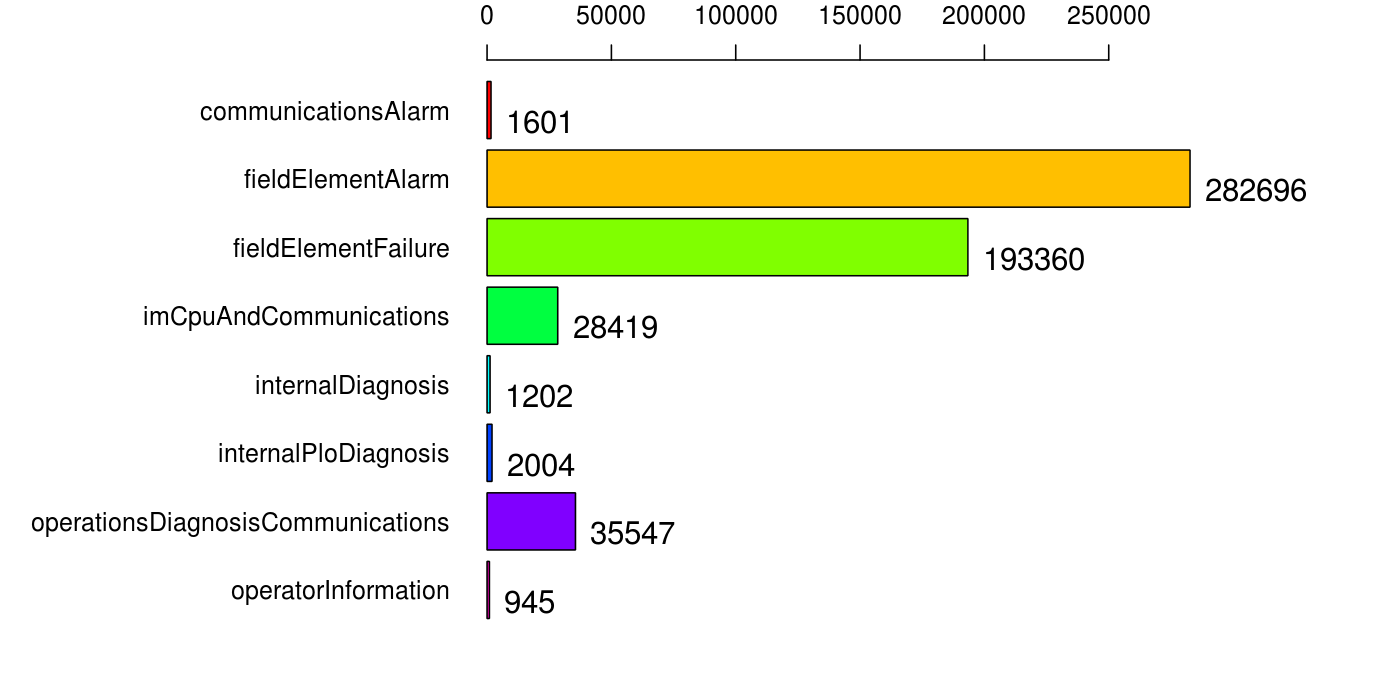
\includegraphics[width=\textwidth]{img/clusters_alb.png}
\caption{Clusters and their size for Albacete station} \label{fig:clusters_alb}
\end{figure}

\begin{figure}[hbtp]
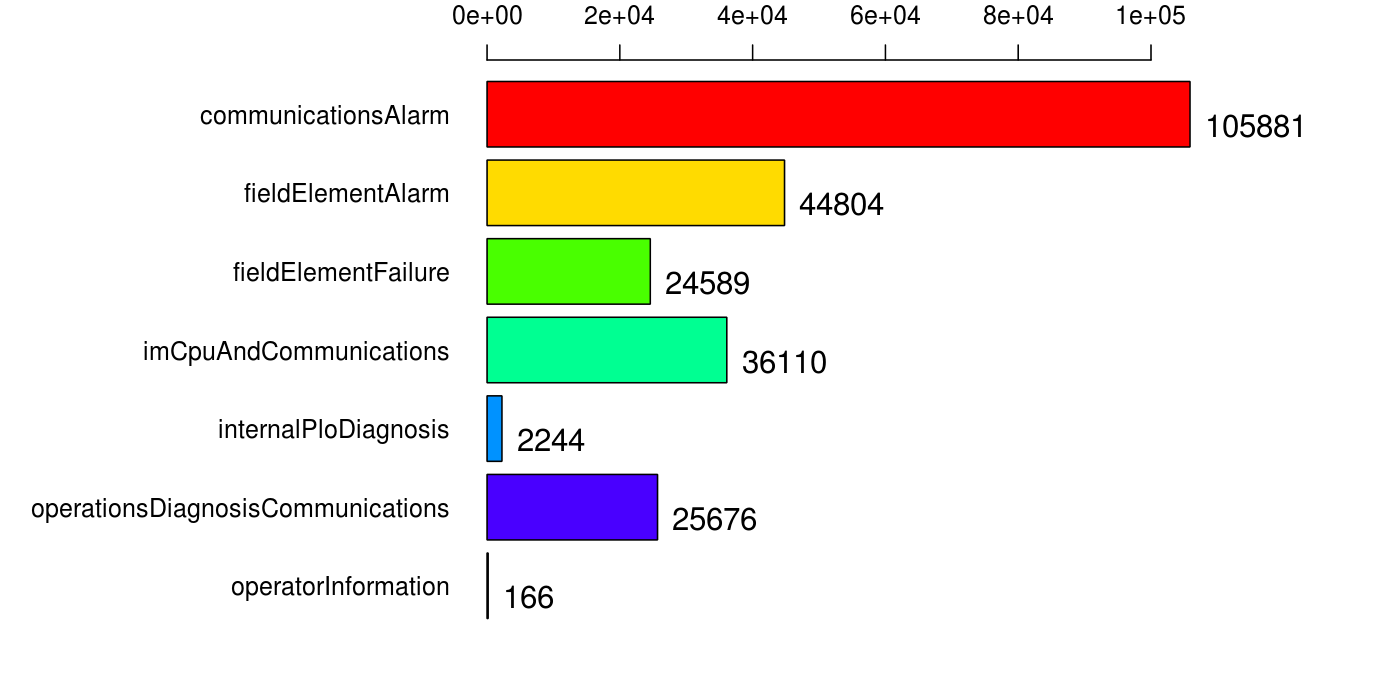
\includegraphics[width=\textwidth]{img/clusters_ant.png}
\caption{Clusters and their size for Antequera station} \label{fig:clusters_ant}
\end{figure}

\begin{figure}[hbtp]
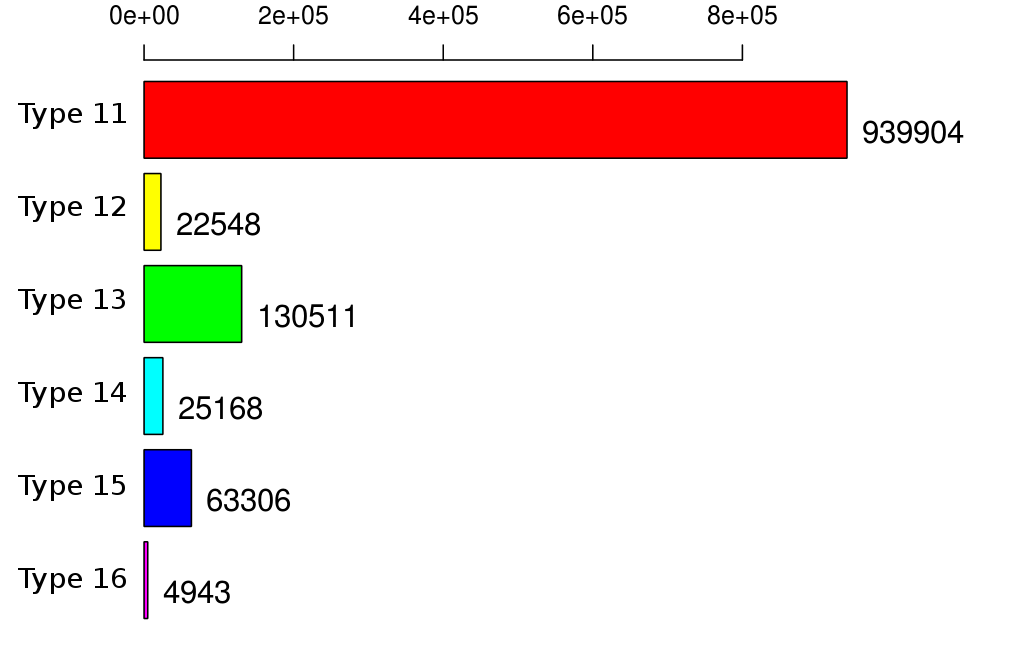
\includegraphics[width=\textwidth]{img/clusters_seg.png}
\caption{Clusters and their size for Segovia station} \label{fig:clusters_seg}
\end{figure}

\begin{figure}[hbtp]
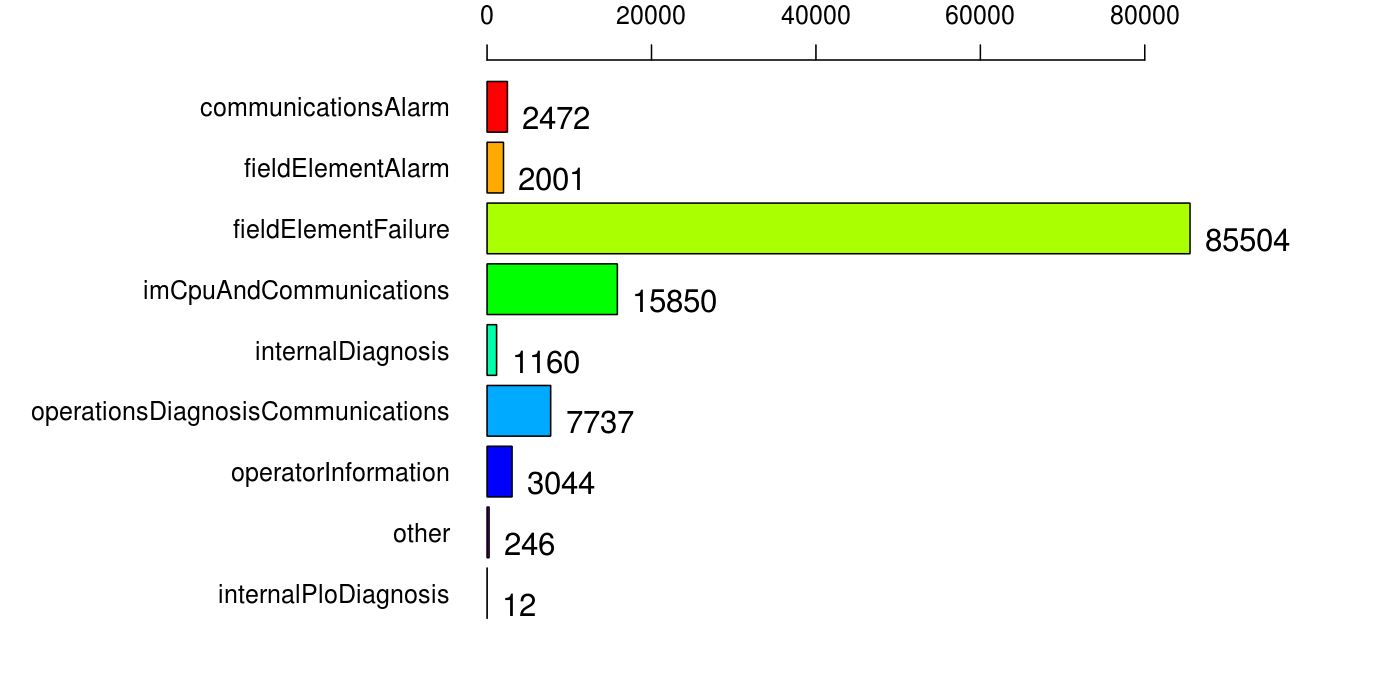
\includegraphics[width=\textwidth]{img/clusters_sev.png}
\caption{Clusters and their size for Sevilla station} \label{fig:clusters_sev}
\end{figure}


\begin{table}
\begin{center}
\begin{tabular}{|c|c|c|}
\hline \headcell{Cluster size} & \headcell{Maximum number of antecedents} & \headcell{Minimum support} \\ 
\hline 
$<$ 10.000 & 7 & 0.01 \\ 
\hline 
10.000 - 50.000 & 5 & 0.1 \\ 
\hline 
50.000 - 100.000 & 5 & 0.2 \\ 
\hline 
$>$100.000 & 5 & 0.3 \\ 
\hline 

\end{tabular} 
\caption{Search depth parameters for different cluster sizes} \label{tab:thumbrule}
\end{center}
\end{table}

\subsection{Grouping similar physical elements}
\label{sec:group_elements}
As a second method, we will try and group alarms by the element which raises them. For our \emph{empty intersection} rule to be followed, we will need to make groups which gather \emph{all} the elements which can raise the same type of alarms. Unfortunately, information on the physical elements which raise the alarms is not directly tabulated and available in the provided databases. The corresponding element is instead included as part of the message shown to the operator, sometimes along with other parameters, and therefore this classification cannot be directly made.

In order to achieve this, we will check, for all the different possible events, their associated \emph{ADDITIONAL\_INFOS} field, which depends on (but not corresponds to) the raising elements. By looking for similar naming patterns on said field, we might be able to find a way to perform this desired way of clustering. Most of the groups did not follow evident patterns at first sight, but after analysing all their relations with different alarms, we were able to come with several clusters. The created groups for Antequera station can be seen in table~\ref{tab:custom_clusters}. For example, \emph{ADDITIONAL\_INFOS} fields of the form E1, E2, E3... always were found in lights-related alarms, same as for the form R1, R2, R3... and therefore all the events falling into these conditions will be clustered into the \emph{lights} cluster.

These groups do not follow any official categorisation made by Thales' engineers. Although an index of physical elements existed and was available, its relation with the alarms in the database was not direct. Furthermore, what we want to achieve is groups of elements which are likely to raise similar elements (and to follow similar patterns in their occurence) and therefore we do not need these groups to be actually made by exact classification of the types of elements.

Comparison of results with and without this kind of clustering can be seen in figure~\ref{fig:group_vs_nogroup}. The number of high-precision rules significantly increases by using this kind of clustering. Further comments on the results can be found in section~\ref{sec:results}.

This process, however, must be made manually looking for different patterns and elements which seem to raise the same type of events. Therefore, it is a very time consuming process and its not suitable for being applied systematically to all datasets. The provided data corresponds to the station of Antequera, for which we have performed the procedure in order to evaluate its possible benefits. In order for this to be suitable for general application, additional info should be provided in datasets which could allow faster automatic grouping.

\begin{table}
\begin{center}
\begin{tabular}{|c|c|c|}
\hline \headcell{ADDITIONAL\_INFOS pattern} & \headcell{Cluster} \\ 
\hline 
A00, A01, A02... & Switches \\ 
\hline 
10, 11, 12... 140 & Lights \\ 
\hline 
E1, E2, E3, E4 ... & Lights \\ 
\hline 
S1/1, S1/2 ... & Lights \\ 
\hline 
R1, R2, R3 ... & Lights \\ 
\hline 
M1, M2, M3 ... & Lights \\ 
\hline 
A|XX|XX & Communications \\ 
\hline 
B|XX|XX & Communications \\ 
\hline 
IM|XX|XX & Communications \\ 
\hline 
EC|XX|XX & Communications \\ 
\hline
EN-A, EN-B, EN-M & Electric network and power supply \\ 
\hline   
ALI\_XXX & Electric network and power supply \\ 
\hline   
Alimentacion XXX & Electric network and power supply \\ 
\hline   
V1, V2 ... & Rail tracks \\ 
\hline   

\end{tabular} 
\caption{Clusters found for different patterns in ADDITIONAL\_INFOS field} \label{tab:custom_clusters}
\end{center}
\end{table}

\begin{figure}[hbtp]
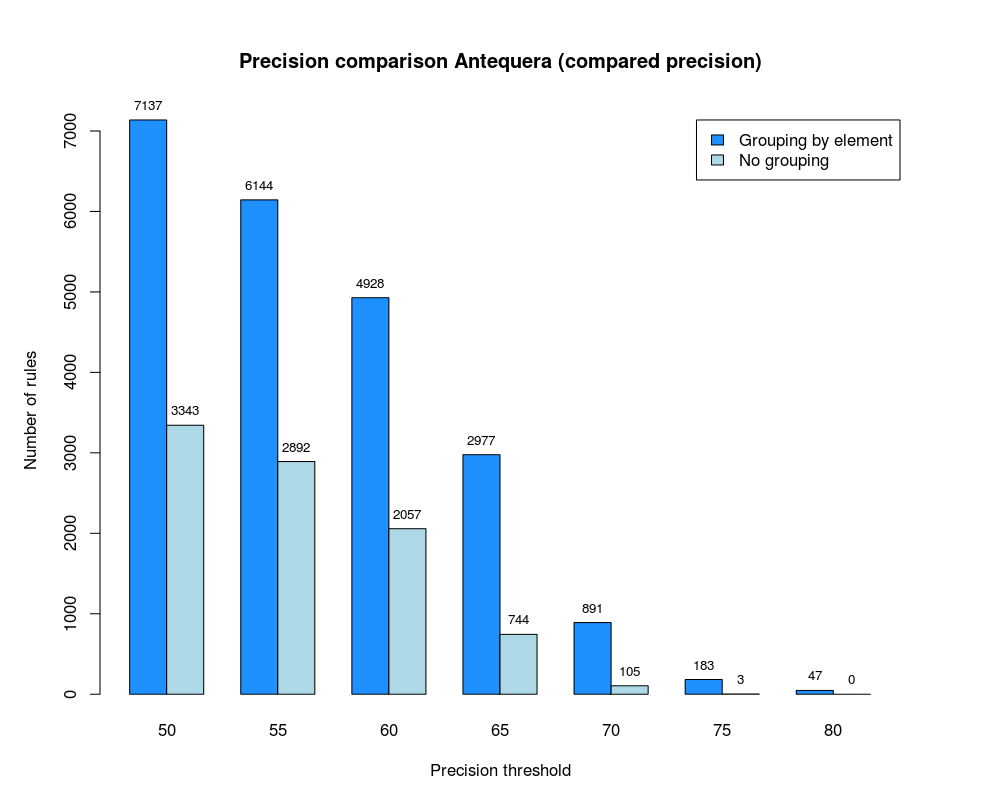
\includegraphics[width=\textwidth]{img/group_vs_nogroup.png}
\caption{Number of rules by precision before and after grouping by similar elements} \label{fig:group_vs_nogroup}
\end{figure}

\clearpage
\section{Results}
\label{sec:results}
In this section we will make a deep insight on the obtained data. Our goal was to generate different rulesets for each of our maintenance stations, each of them covering different time windows. Specifically, we have studied three different time windows: one day, two days and one week. This defines the observation period for our predictive work, which means not only the time span we will use as antecedents for our rules but also the time window within which our prediction can occur.

The results are very different depending on which station and time period we chose. In this section we will analyse the results obtained for each of them from different perspectives.

\subsection{Description of obtained rulesets}
\label{sec:desc_results}
The result of the previous work described in section~\ref{sec:assoc_rules} comes in the form of a set of association rules. These \emph{rule sets} contain a list of all the association rules found, along with their performance value calculed by the \emph{K-fold-CV} procedure as defined in section~\ref{sec:validation_evaluation}. The obtained rulesets and the number of rules they contain can be seen in table~\ref{tab:numrules}.

These sets contain all the information obtained from the procedure defined in section~\ref{sec:assoc_rules}. It is important to note that not all of them will be useful in order to implement a predictive system, as their precision is sometimes as low as 5\%. The threshold for a rule to be useful needs to be defined by maintenance workers who know the associated costs of maintenance tasks required to handle raised predictions before knowing if they will actually happen. If some event needs a significantly high amount of money to be avoided we will probably want to be \emph{very} confident about our precisions regarding that kind of event before investing resources on preventing it.

However, in general terms we can consider a prediction is good when it has more chances of being a right guess than a wrong one. We will therefore set p=0.5 as the point where rules \emph{start} to be useful. Rules with lower precisions are still provided and can be useful for other analysis tasks or further research, but from now on we will disregard them and focus on the \emph{0.5 set} which can be used right away for predictive purposes. These new sets and their size can be seen in table~\ref{tab:numrules_50}. Obviously, the size of the sets reduces drastically when imposing this kind of conditions.

\begin{table}
\begin{center}
\begin{tabular}{|c|c|c|}
\hline \headcell{Station} & \headcell{Time Window} & \headcell{Rules} \\ 
\hline 
Albacete & 1 day & 27522 \\ 
\hline 
Albacete & 7 days & 50281 \\ 
\hline 
Antequera & 1 day & 39214 \\ 
\hline 
Segovia & 1 day & 113 \\ 
\hline 
Segovia & 2 days & 72 \\ 
\hline
Segovia & 7 days & 133 \\ 
\hline 
Sevilla & 1 day & 8091 \\ 
\hline 

\end{tabular} 
\caption{Size of obtained rule sets for each station and time window} \label{tab:numrules}
\end{center}
\end{table}

\begin{table}
\begin{center}
\begin{tabular}{|c|c|c|}
\hline \headcell{Station} & \headcell{Time Window} & \headcell{Rules} \\ 
\hline 
Albacete & 7 days & 9 \\ 
\hline 
Antequera & 1 day & 7104 \\ 
\hline 
Segovia & 1 day & 31 \\ 
\hline 
Segovia & 2 days & 30 \\ 
\hline
Segovia & 7 days & 48 \\ 
\hline 
Sevilla & 1 day & 242 \\ 
\hline 

\end{tabular} 
\caption{Number of rules for each set setting a threshold of 50\% precision} \label{tab:numrules_50}
\end{center}
\end{table}



At this point, it is important to remember the decisions taken in terms of search depth and data subsetting as mentioned in sections~\ref{sec:search_parameters} and~\ref{sec:dataclustering}. In these terms, rule sets for some of the stations and time windows could not be generated with our available computation capabilities. A better server or algorithm optimisation would be required in order to obtain result sets for these cases.

\subsection{Number of rules against precision}
\label{sec:rules_vs_prec}
As we have seen in section~\ref{sec:desc_results}, the amount of rules decreases significantly if we impose strict conditions for their validity. In this section we will perform a deeper analysis on how amount of rules vary when setting different thresholds. For this purpose, we will set different thresholds and check the number of rules complying with this condition. The results are shown in tables \ref{tab:numrules_thresh_albacete7}, \ref{tab:numrules_thresh_antequera1}, \ref{tab:numrules_thresh_segovia1}, \ref{tab:numrules_thresh_segovia2}, \ref{tab:numrules_thresh_segovia7} and \ref{tab:numrules_thresh_sevilla1}. As expected, the number of rules increases exponentially when decreasing the threshold. For better visualization, these amounts for the \emph{$>50\%$ subsets} are represented in figures~\ref{fig:precision_alb7}, \ref{fig:precision_ant1}, \ref{fig:precision_seg1}, \ref{fig:precision_seg2}, \ref{fig:precision_seg7} and \ref{fig:precision_sev1}.

\begin{table}
\begin{center}
\begin{tabular}{|c|c|c|}
\hline \headcell{Threshold} & \headcell{Number of rules} \\ 
\hline 
0.05 & 44620 \\ 
\hline 
0.10 & 38007 \\ 
\hline 
0.20 & 4060 \\ 
\hline 
0.30 & 30 \\ 
\hline
0.40 & 27 \\ 
\hline 
0.50 & 9 \\ 
\hline 
0.60 & 8 \\ 
\hline 

\end{tabular} 
\caption{Number of rules for different thresholds in Albacete (7 days)} \label{tab:numrules_thresh_albacete7}
\end{center}
\end{table}

\begin{table}
\begin{center}
\begin{tabular}{|c|c|c|}
\hline \headcell{Threshold} & \headcell{Number of rules} \\ 
\hline 
0.05 & 31846 \\ 
\hline 
0.10 & 28338 \\ 
\hline 
0.20 & 21566 \\ 
\hline 
0.30 & 15829 \\ 
\hline
0.40 & 10876 \\ 
\hline 
0.50 & 7137 \\ 
\hline 
0.60 & 4928 \\ 
\hline 
0.70 & 891 \\ 
\hline 
0.80 & 47 \\ 
\hline 

\end{tabular} 
\caption{Number of rules for different thresholds in Antequera (1 day)} \label{tab:numrules_thresh_antequera1}
\end{center}
\end{table}

\begin{table}
\begin{center}
\begin{tabular}{|c|c|c|}
\hline \headcell{Threshold} & \headcell{Number of rules} \\ 
\hline 
0.05 & 106 \\ 
\hline 
0.10 & 95 \\ 
\hline 
0.20 & 72 \\ 
\hline 
0.30 & 44 \\ 
\hline
0.40 & 33 \\ 
\hline 
0.50 & 31 \\ 
\hline 
0.60 & 30 \\ 
\hline 
0.70 & 24 \\ 
\hline 
0.80 & 12 \\ 
\hline 

\end{tabular} 
\caption{Number of rules for different thresholds in Segovia (1 day)} \label{tab:numrules_thresh_segovia1}
\end{center}
\end{table}

\begin{table}
\begin{center}
\begin{tabular}{|c|c|c|}
\hline \headcell{Threshold} & \headcell{Number of rules} \\ 
\hline 
0.05 & 69 \\ 
\hline 
0.10 & 66 \\ 
\hline 
0.20 & 56 \\ 
\hline 
0.30 & 40 \\ 
\hline
0.40 & 31 \\ 
\hline 
0.50 & 30 \\ 
\hline 
0.60 & 14 \\ 
\hline 

\end{tabular} 
\caption{Number of rules for different thresholds in Segovia (2 days)} \label{tab:numrules_thresh_segovia2}
\end{center}
\end{table}

\begin{table}
\begin{center}
\begin{tabular}{|c|c|c|}
\hline \headcell{Threshold} & \headcell{Number of rules} \\ 
\hline 
0.05 & 128 \\ 
\hline 
0.10 & 125 \\ 
\hline 
0.20 & 92 \\ 
\hline 
0.30 & 75 \\ 
\hline
0.40 & 64 \\ 
\hline 
0.50 & 48 \\ 
\hline 
0.60 & 35 \\ 
\hline 
0.70 & 30 \\ 
\hline 
0.80 & 25 \\ 
\hline 
0.90 & 4 \\ 
\hline 

\end{tabular} 
\caption{Number of rules for different thresholds in Segovia (7 days)} \label{tab:numrules_thresh_segovia7}
\end{center}
\end{table}

\begin{table}
\begin{center}
\begin{tabular}{|c|c|c|}
\hline \headcell{Threshold} & \headcell{Number of rules} \\ 
\hline 
0.05 & 6730 \\ 
\hline 
0.10 & 2832 \\ 
\hline 
0.20 & 2357 \\ 
\hline 
0.30 & 1799 \\ 
\hline
0.40 & 642 \\ 
\hline 
0.50 & 246 \\ 
\hline 
0.60 & 78 \\ 
\hline 
0.70 & 2 \\ 
\hline 

\end{tabular} 
\caption{Number of rules for different thresholds in Sevilla (1 day)} \label{tab:numrules_thresh_sevilla1}
\end{center}
\end{table}

\begin{figure}[hbtp]
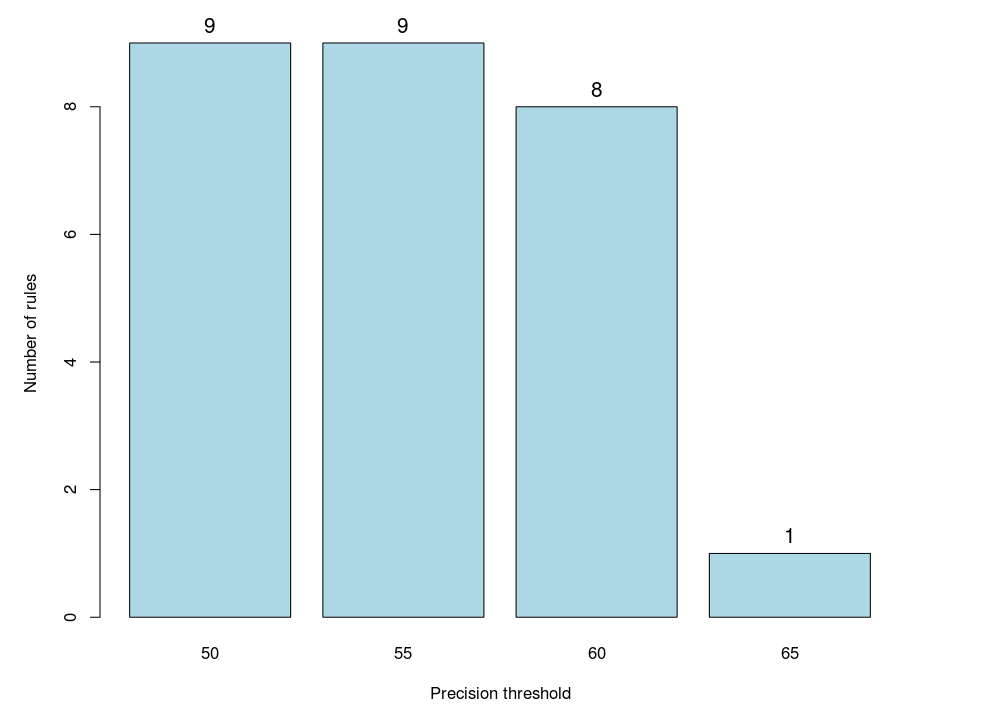
\includegraphics[width=\textwidth]{img/precision_alb7.png}
\caption{Number of rules for different thresholds in Albacete (7 days)} \label{fig:precision_alb7}
\end{figure}

\begin{figure}[hbtp]
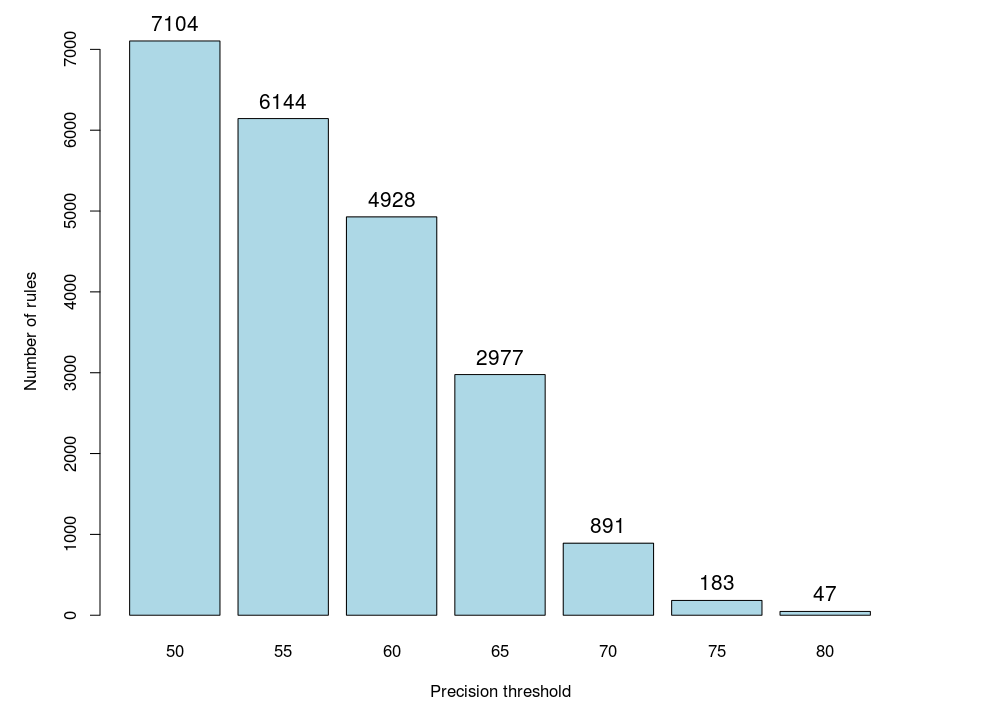
\includegraphics[width=\textwidth]{img/precision_ant1.png}
\caption{Number of rules for different thresholds in Antequera (1 day)} \label{fig:precision_ant1}
\end{figure}

\begin{figure}[hbtp]
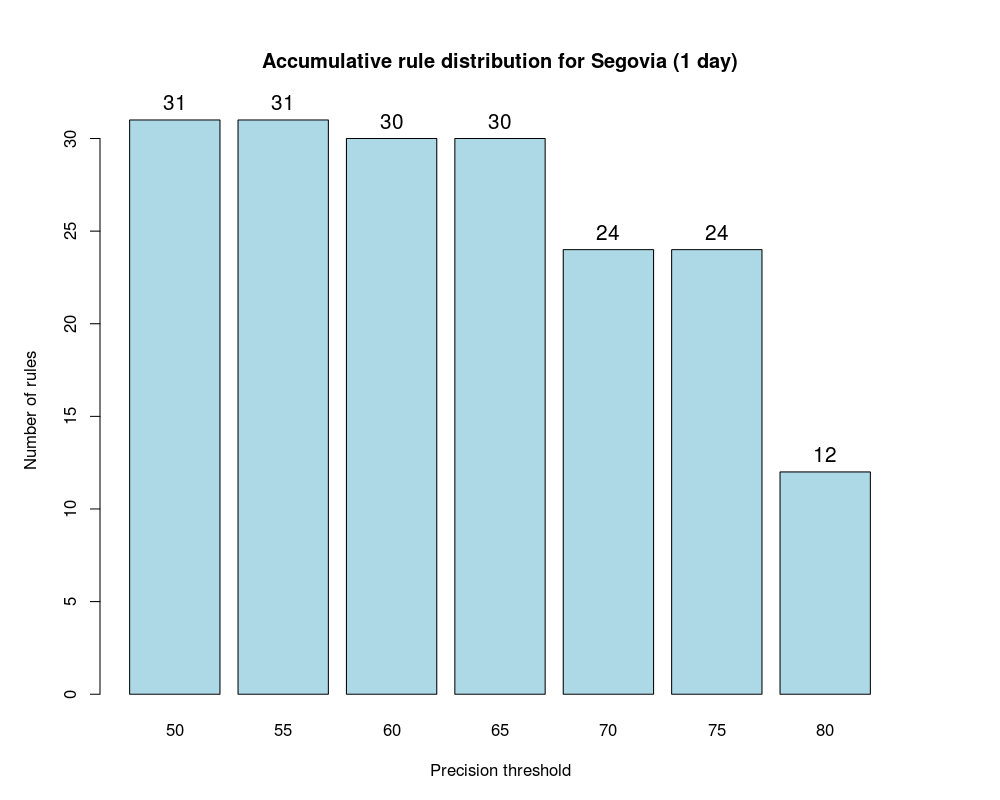
\includegraphics[width=\textwidth]{img/precision_seg1.png}
\caption{Number of rules for different thresholds in Segovia (1 day)} \label{fig:precision_seg1}
\end{figure}

\begin{figure}[hbtp]
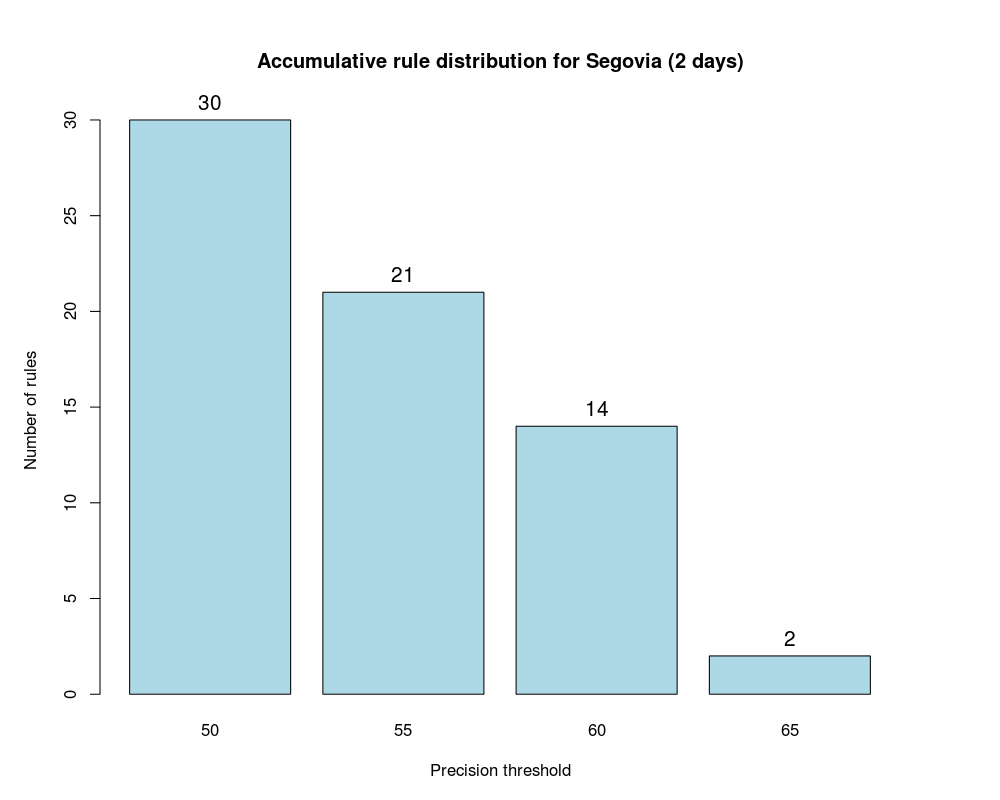
\includegraphics[width=\textwidth]{img/precision_seg2.png}
\caption{Number of rules for different thresholds in Segovia (2 days)} \label{fig:precision_seg2}
\end{figure}

\begin{figure}[hbtp]
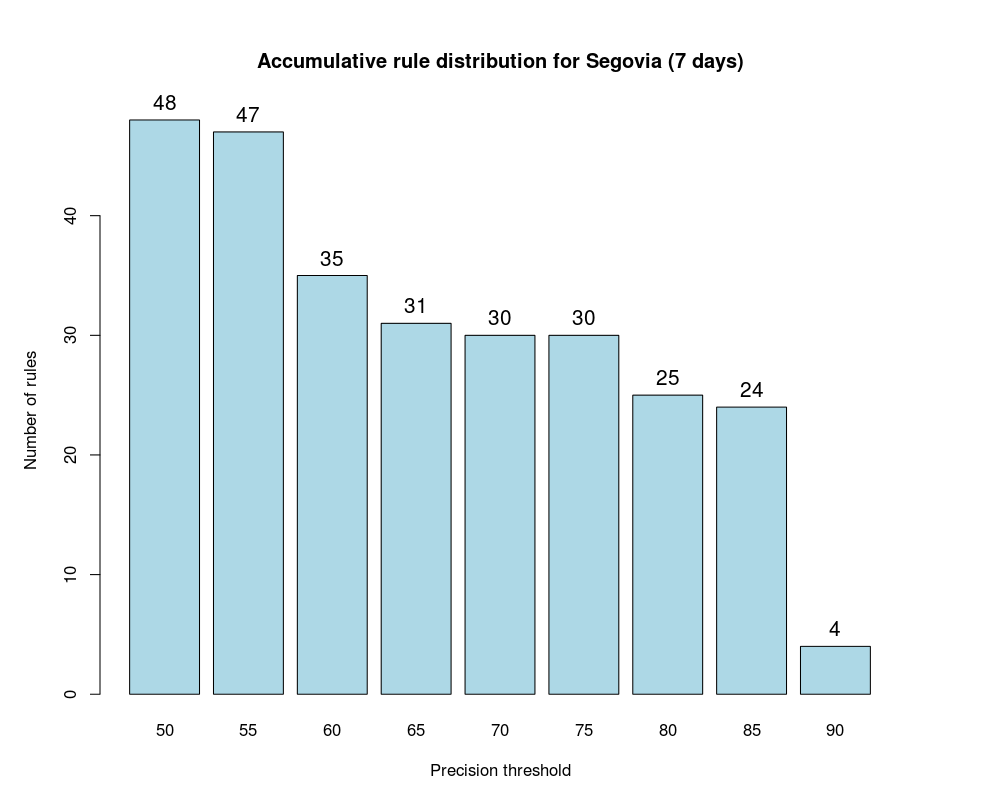
\includegraphics[width=\textwidth]{img/precision_seg7.png}
\caption{Number of rules for different thresholds in Segovia (7 days)} \label{fig:precision_seg7}
\end{figure}

\begin{figure}[hbtp]
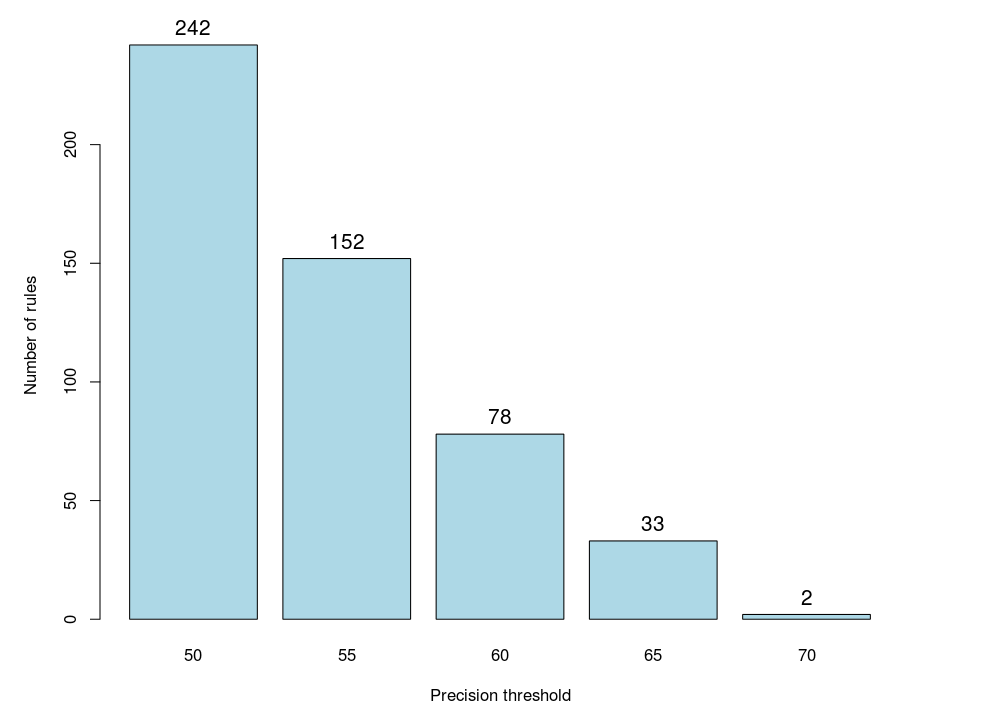
\includegraphics[width=\textwidth]{img/precision_sev1.png}
\caption{Number of rules for different thresholds in Sevilla (1 day)} \label{fig:precision_sev1}
\end{figure}

\clearpage

\subsection{Precision distribution}
\label{sec:precision_distribution}
In section~\ref{sec:rules_vs_prec} we analysed the number of rules we would obtain if we set different precision levels as thresholds to generate different subsets. According to our expectations, we observed a decay in these numbers as we set higher thresholds. However, this decay, although apparently exponential, shows flat zones and other irregularities which would be unexpected at first.

In order to better visualize these anomalities we will graphically represent the precision distribution in form of histograms for the previous sets. These distributions can be seen in figures~\ref{fig:hist_alb7}, \ref{fig:hist_ant1}, \ref{fig:hist_seg1}, \ref{fig:hist_seg2}, \ref{fig:hist_seg7} and \ref{fig:hist_sev1}.

In these histograms we can see that the distribution does not grow exponentially as we lower the precision, as we would expect and as we apparently saw in the analysis from section~\ref{sec:rules_vs_prec}. Instead, there are some accumulation points around which precision tends to take values. 

For example, looking at the distribution for Antequera (figure~\ref{fig:hist_ant1}) we see that there are more rules with precisions between 0.65 and 0.70 than between 0.50 and 0.55.

As we do not have large sets of rules for all the stations, performing a deeper analysis of the distributions is not possible. As these kind of irregularities appear for all the studied cases, it is very unlikely that they are caused just by chance. However, the causes and possible implications of these distributions cannot be infered at this point and would require further research.

\begin{figure}[hbtp]
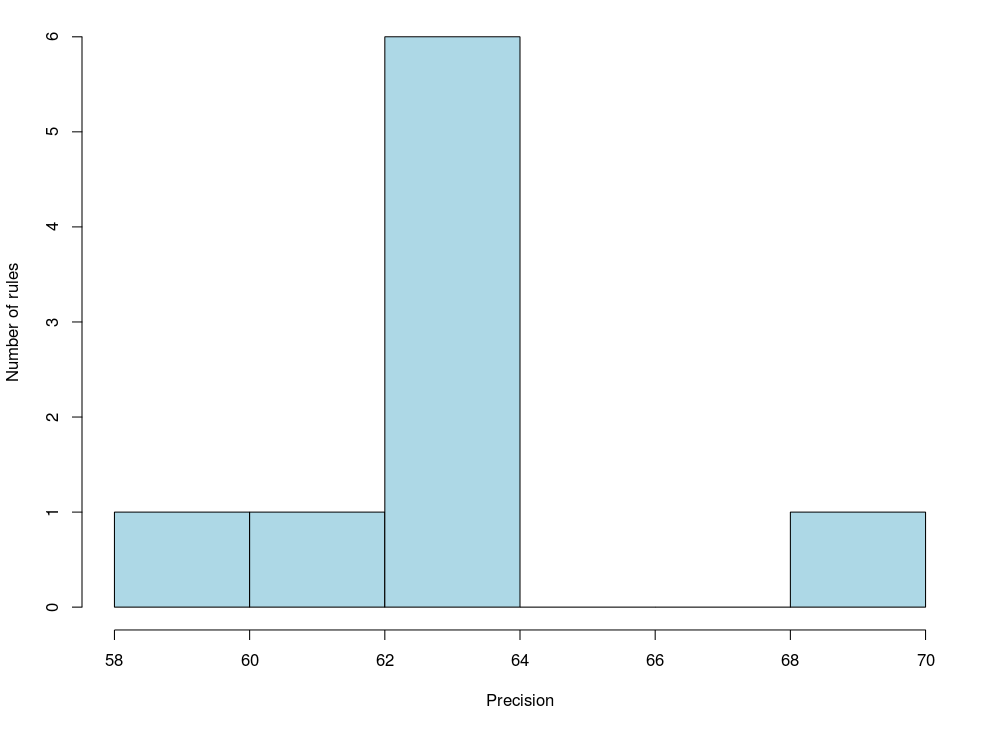
\includegraphics[width=\textwidth]{img/hist_alb7.png}
\caption{Rule distribution by precision in Albacete (7 days)} \label{fig:hist_alb7}
\end{figure}

\begin{figure}[hbtp]
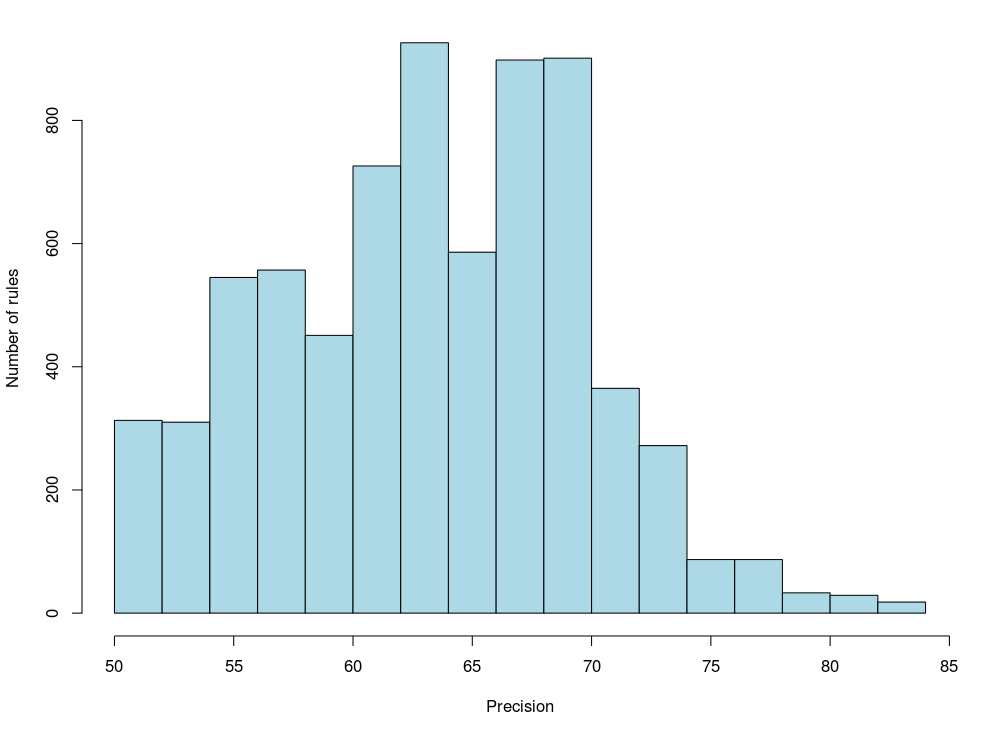
\includegraphics[width=\textwidth]{img/hist_ant1.png}
\caption{Rule distribution by precision in Antequera (1 day)} \label{fig:hist_ant1}
\end{figure}

\begin{figure}[hbtp]
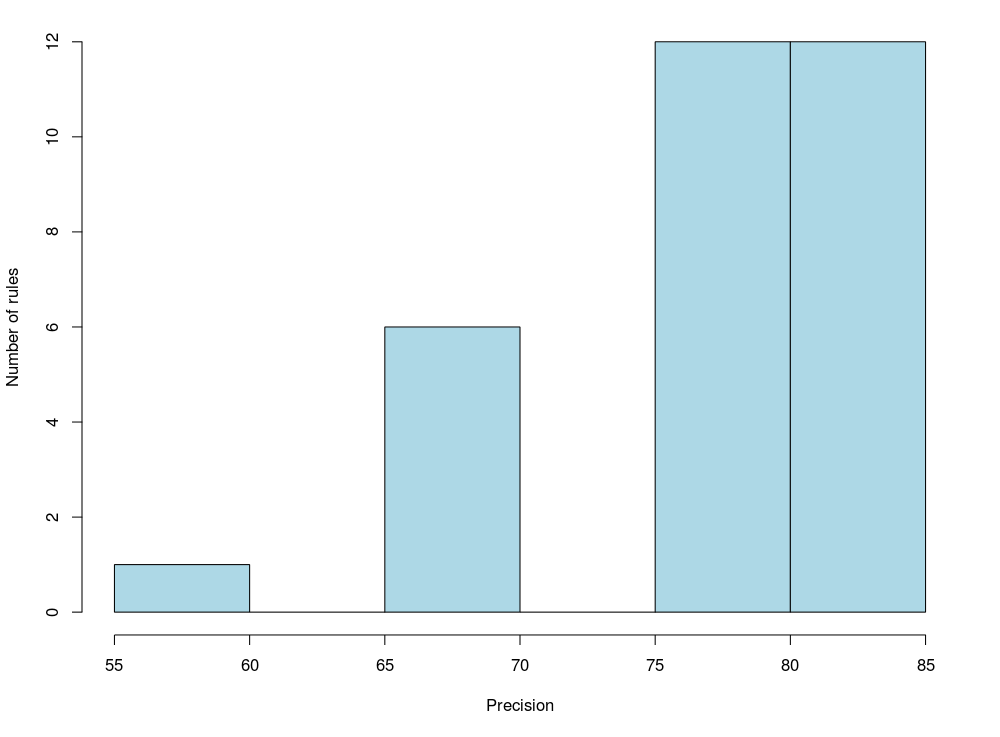
\includegraphics[width=\textwidth]{img/hist_seg1.png}
\caption{Rule distribution by precision in Segovia (1 day)} \label{fig:hist_seg1}
\end{figure}

\begin{figure}[hbtp]
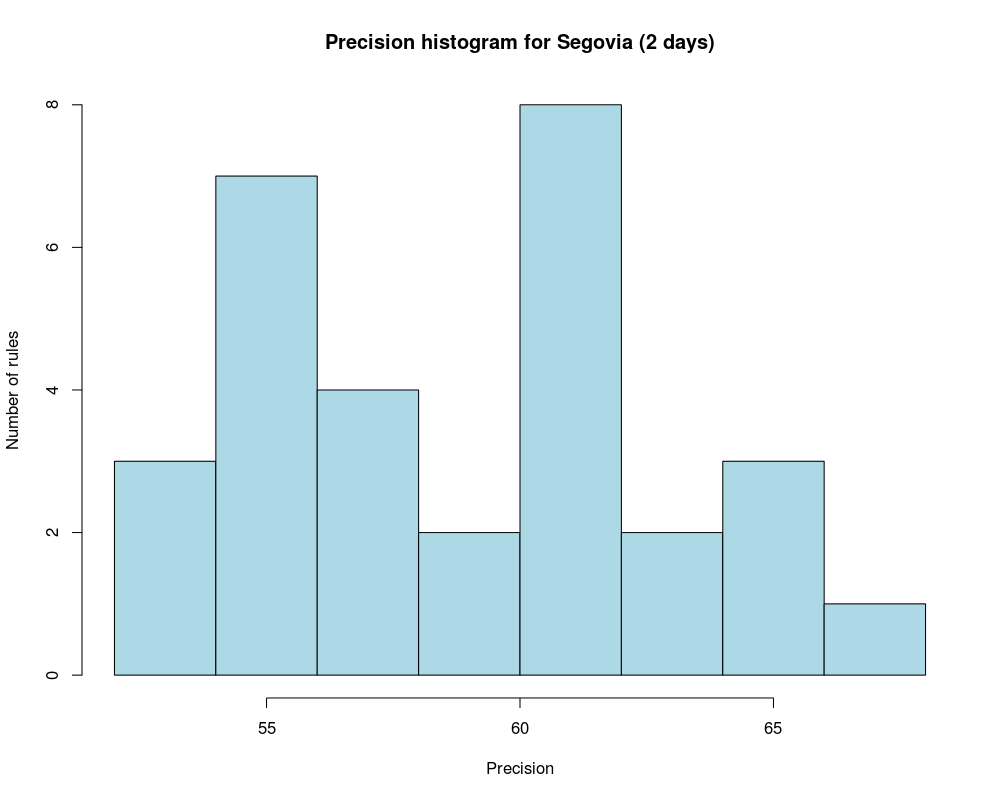
\includegraphics[width=\textwidth]{img/hist_seg2.png}
\caption{Rule distribution by precision in Segovia (2 days)} \label{fig:hist_seg2}
\end{figure}

\begin{figure}[hbtp]
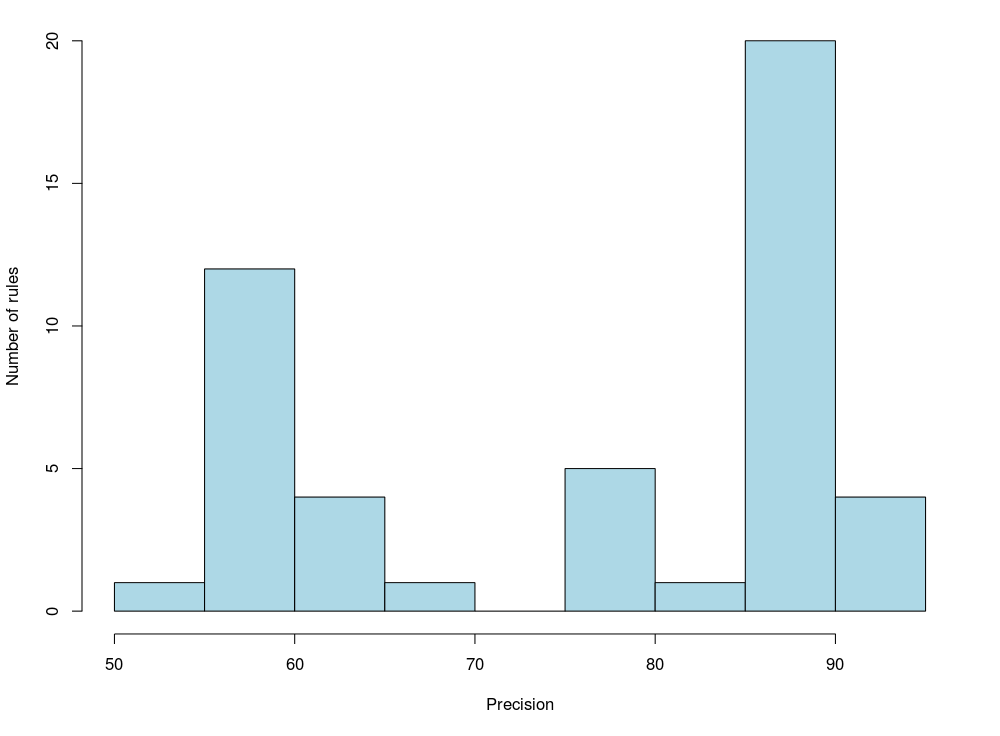
\includegraphics[width=\textwidth]{img/hist_seg7.png}
\caption{Rule distribution by precision in Segovia (7 days)} \label{fig:hist_seg7}
\end{figure}

\begin{figure}[hbtp]
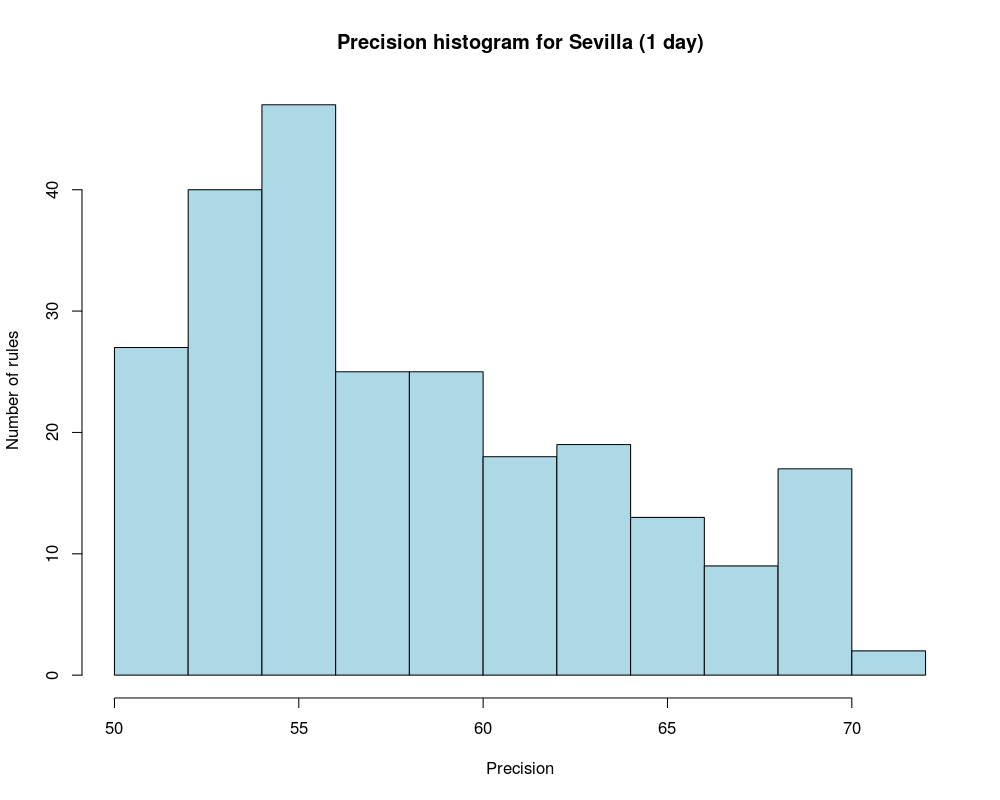
\includegraphics[width=\textwidth]{img/hist_sev1.png}
\caption{Rule distribution by precision in Sevilla (1 day)} \label{fig:hist_sev1}
\end{figure}

\subsection{Predictable events by category}
As we mentioned in section~\ref{sec:using_event_type}, one of the methods followed in order to being able to perform deep searches on our data was clustering by event types. This unavoidably leads to differences on the achievable performance for each of the different event types. This is caused not only by the different search depths which we were able to use in each of the different groups, but also by the individual nature of each of the event types: events in some of the clusters may be more likely to be related to others in the same cluster while for other types these relations may be more likely to be found to events in other clusters. 

In order to analyse the effect of this clustering in the obtained results, we will analyse the category of the events the rules predict. This is, we will analyse the event type of the consequent of our rules. This distribution can be seen in figures \ref{fig:conseqtypes_alb7}, \ref{fig:conseqtypes_ant1}, \ref{fig:conseqtypes_seg1}, \ref{fig:conseqtypes_seg2}, \ref{fig:conseqtypes_seg7} and \ref{fig:conseqtypes_sev1}.

We can see a completely uneven distribution in terms of rule generation for each event type. This is likely to be caused by two facts: nature of the events themselves (how unpredictable or related to other events they are) and frequency adequation (events which happen too often instead of only in specific situations might be harder to predict). Also, the different limit on search depth we were able to impose for the different groups also vastly affects results in this direction.

It is specially interesting the situation in \emph{Antequera}, where we performed an alternative clustering method as mentioned in \ref{sec:group_elements}. In this station, we observe that all the rules fall into the category of \emph{FieldElementFailure} and \emph{Operation diagnosis communications}. Both groups of rules are quite similar in size, although the occurence of those alarm types in the whole database is significantly different. This indicates that this kind of clustering might significantly help in order to obtain more uniform results for all the event types.

\begin{figure}[hbtp]
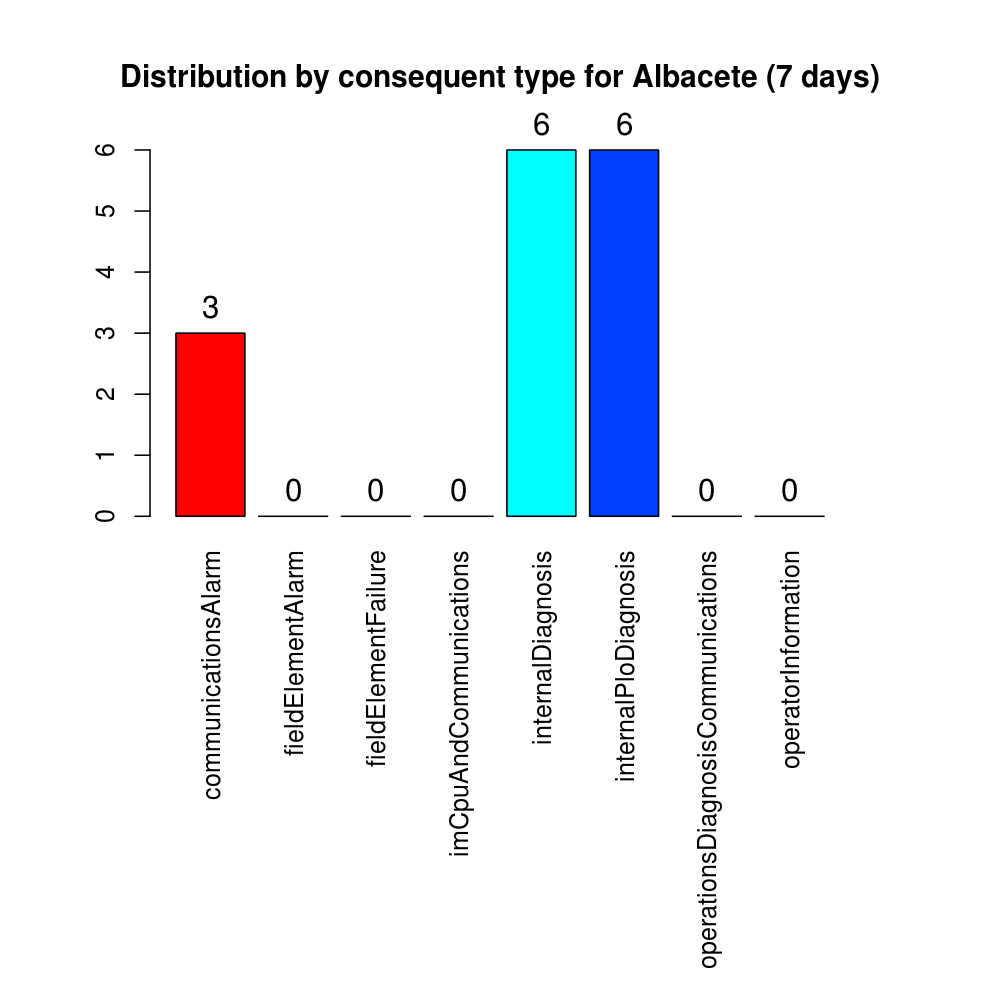
\includegraphics[width=\textwidth]{img/conseqtypes_alb7.png}
\caption{Rule distribution by consequent type in Albacete (7 days)} \label{fig:conseqtypes_alb7}
\end{figure}

\begin{figure}[hbtp]
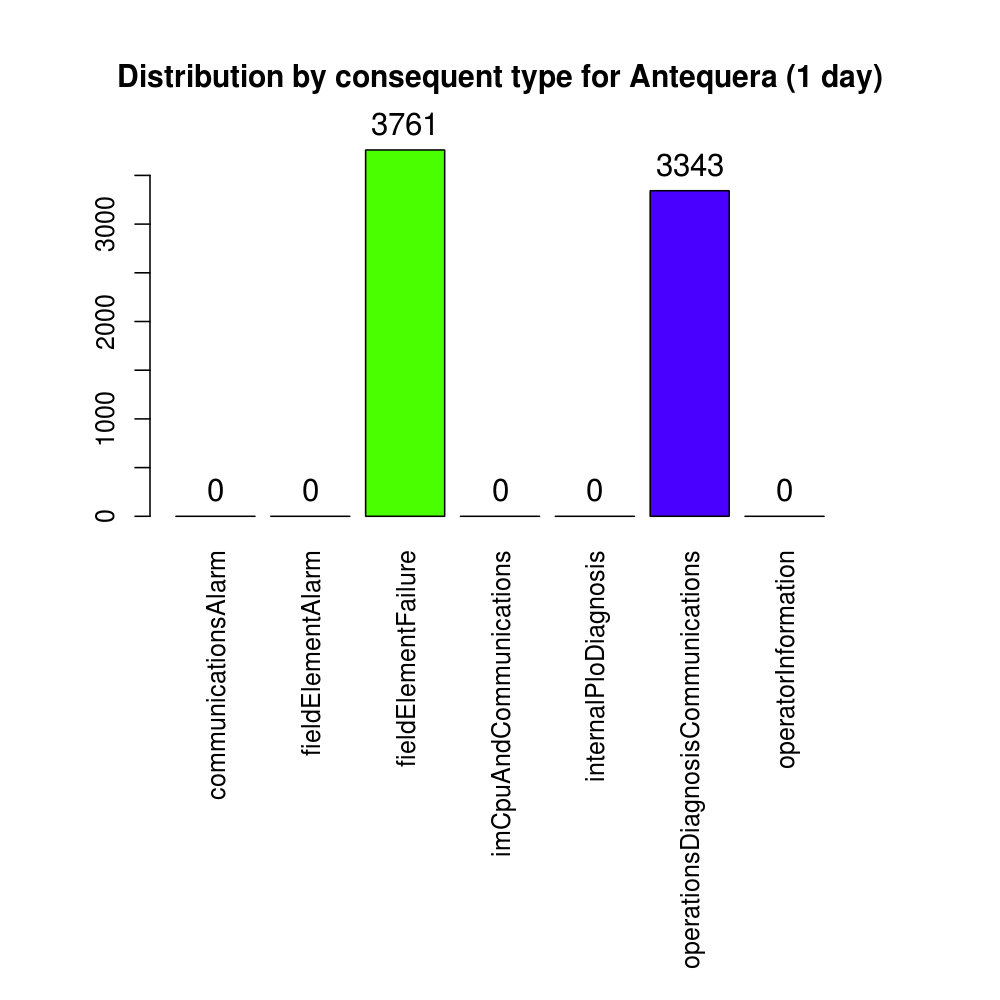
\includegraphics[width=\textwidth]{img/conseqtypes_ant1.png}
\caption{Rule distribution by consequent type in Antequera (1 day)} \label{fig:conseqtypes_ant1}
\end{figure}

\begin{figure}[hbtp]
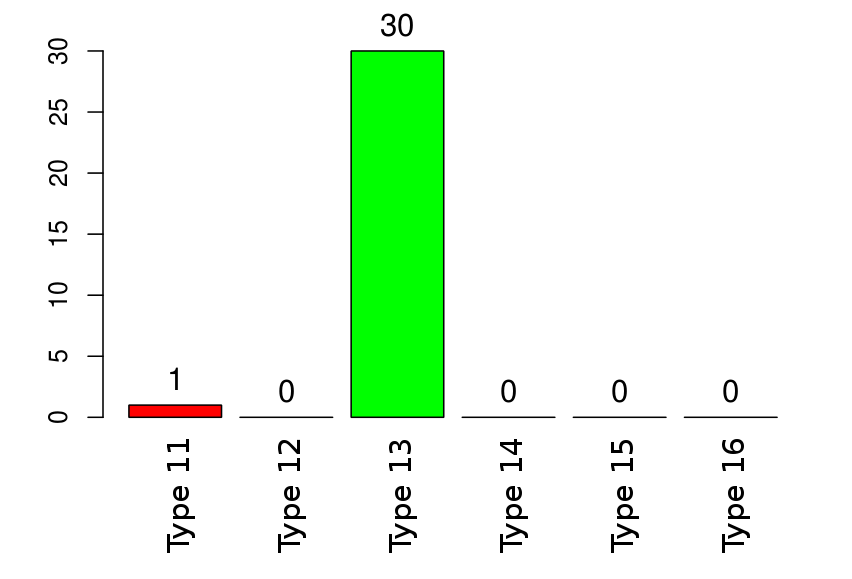
\includegraphics[width=\textwidth]{img/conseqtypes_seg1.png}
\caption{Rule distribution by consequent type in Segovia (1 day)} \label{fig:conseqtypes_seg1}
\end{figure}

\begin{figure}[hbtp]
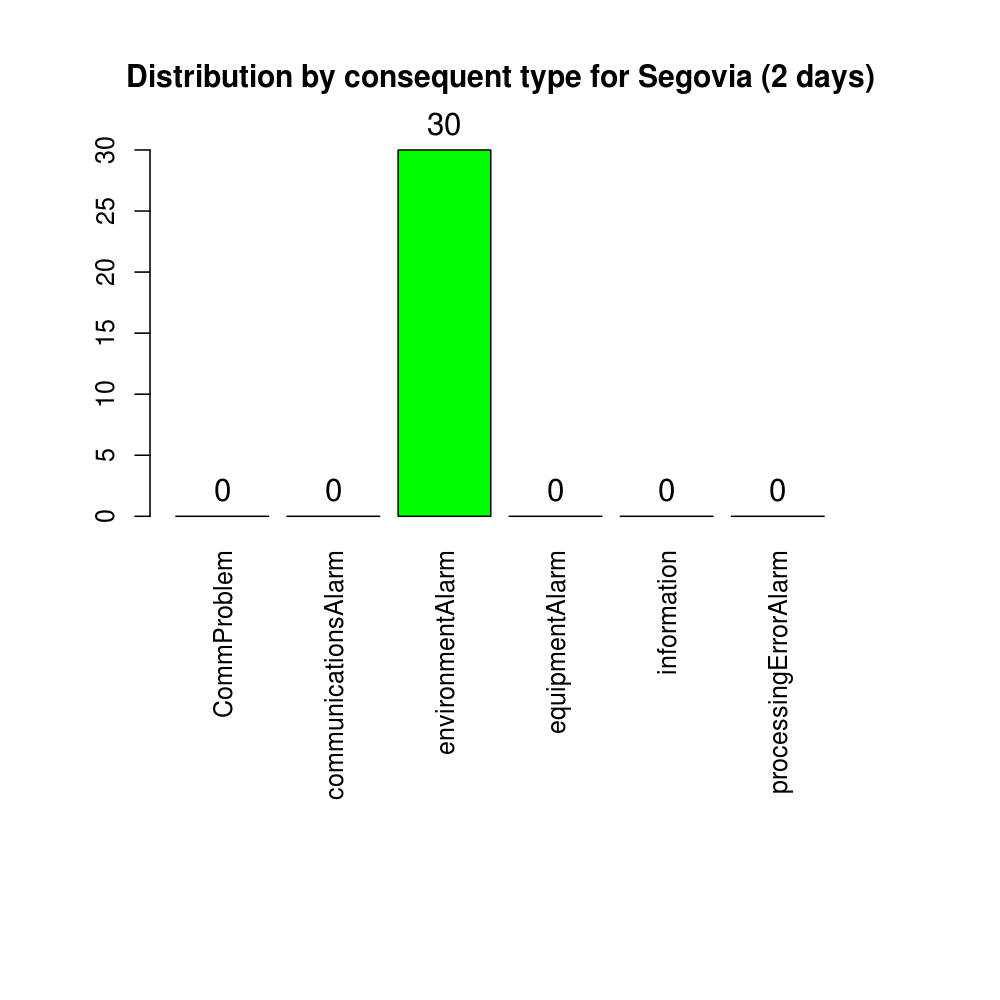
\includegraphics[width=\textwidth]{img/conseqtypes_seg2.png}
\caption{Rule distribution by consequent type in Segovia (2 days)} \label{fig:conseqtypes_seg2}
\end{figure}

\begin{figure}[hbtp]
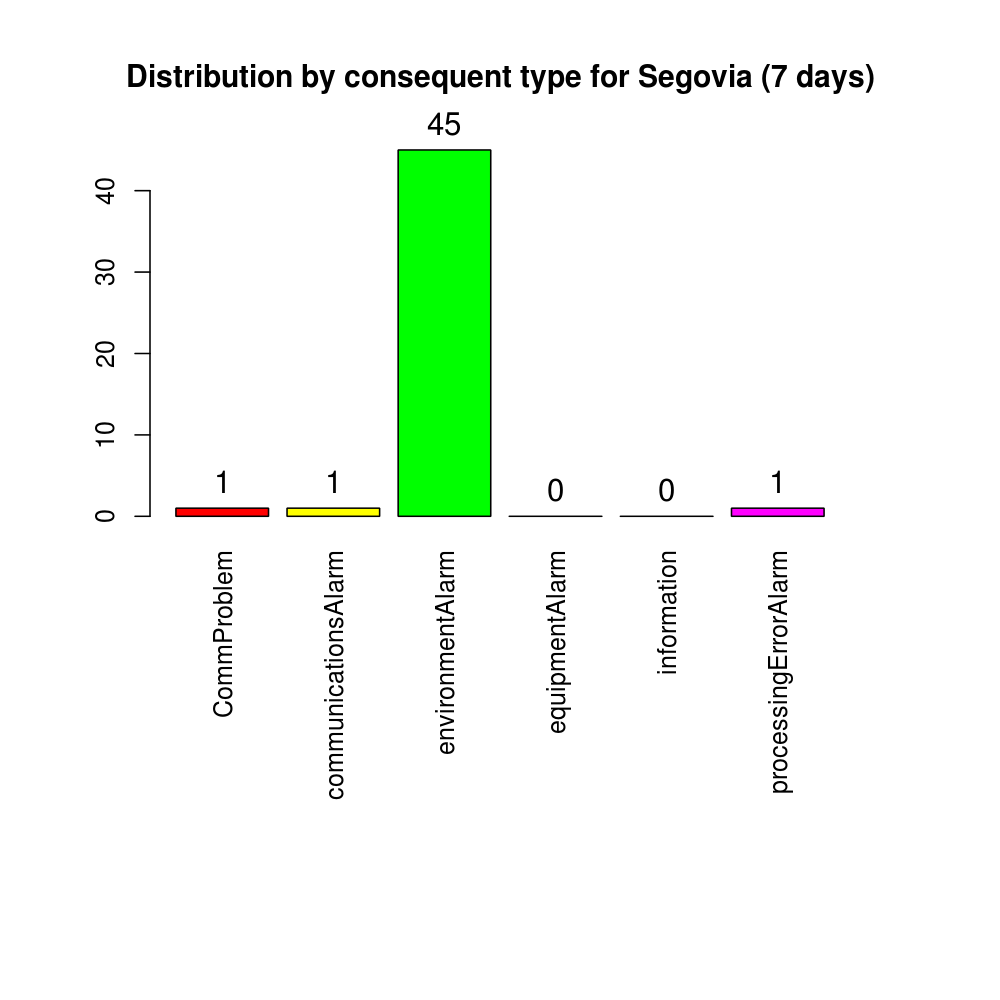
\includegraphics[width=\textwidth]{img/conseqtypes_seg7.png}
\caption{Rule distribution by consequent type in Segovia (7 days)} \label{fig:conseqtypes_seg7}
\end{figure}

\begin{figure}[hbtp]
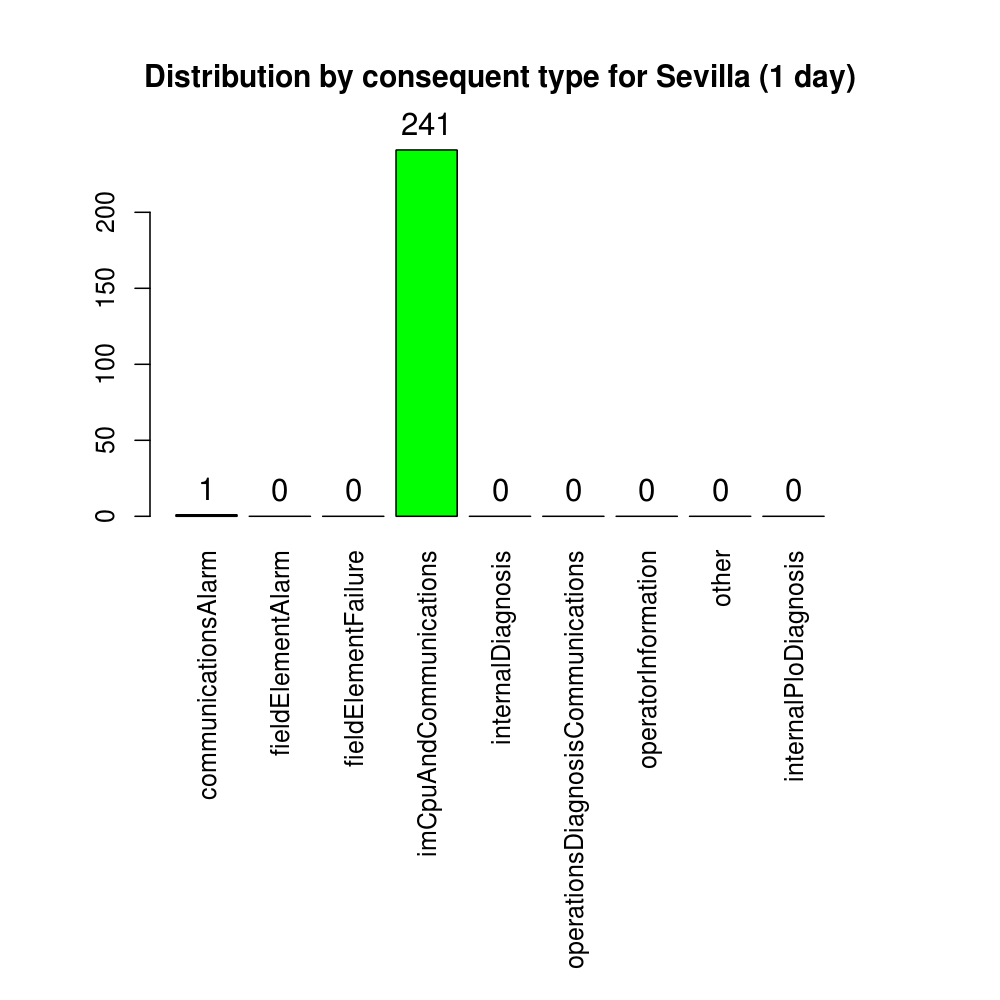
\includegraphics[width=\textwidth]{img/conseqtypes_sev1.png}
\caption{Rule distribution by consequent type in Sevilla (1 day)} \label{fig:conseqtypes_sev1}
\end{figure}


\section{Example scenario}
\label{sec:scenario}

In this section we will analyse the output of our predictive model during a short period of time. We will illustrate the kind of information an operator could obtain from an average period of time. Specifically, we will take a random period of 50 consecutive days for the station of \emph{Antequera}, over which we will perform predictions for the next days.

It is important to note that this example scenario has been obtained using the rule set with precisions higher than 0.50. In a real scenario, an operator could select a higher threshold for predictions or disregard those raised predictions with a low confidence.

\subsection{Predictions raised by event type}
First of all we will observe the number of predictions raised each day of our sample. This will give us an idea of the number of predictions our system would give for an average day. This can be seen in figure~\ref{fig:scenario_pred_categories}.

As we can see, for this station and rule set the number of predictions obtained in an average day is around 20. This does not include repeated predictions (more than one rule which can be fired simultaneously to predict the same event with different confidences).

\begin{figure}[hbtp]
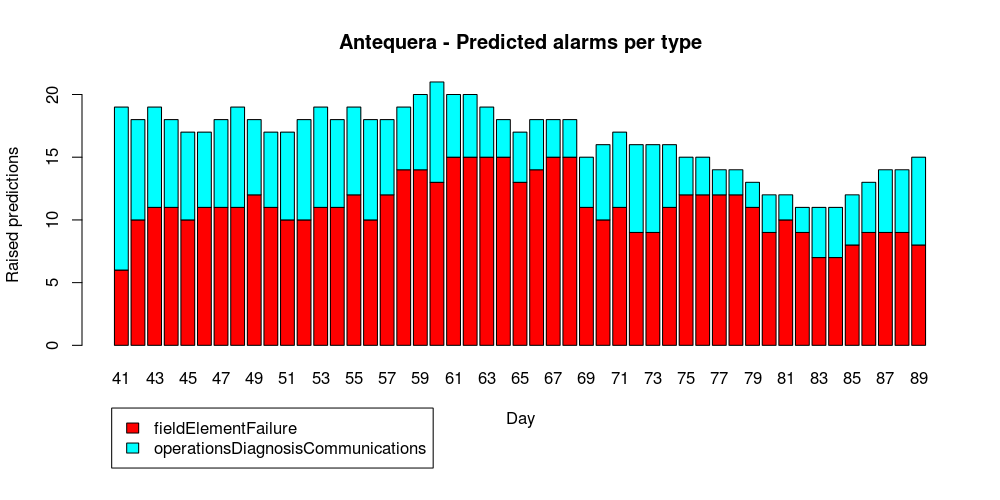
\includegraphics[width=\textwidth]{img/scenario_pred_categories.png}
\caption{Timeline of predictions during a sample period} \label{fig:scenario_pred_categories}
\end{figure}

\subsection{Percentage of events predicted}
The next thing we can analyse is the number of events which happen during an average day which are actually predicted by our system. The result is illustrated in figure~\ref{fig:scenario_pred_notpred}. This value corresponds with what we defined as \emph{recall} in section~\ref{sec:validation_evaluation}.

\begin{figure}[hbtp]
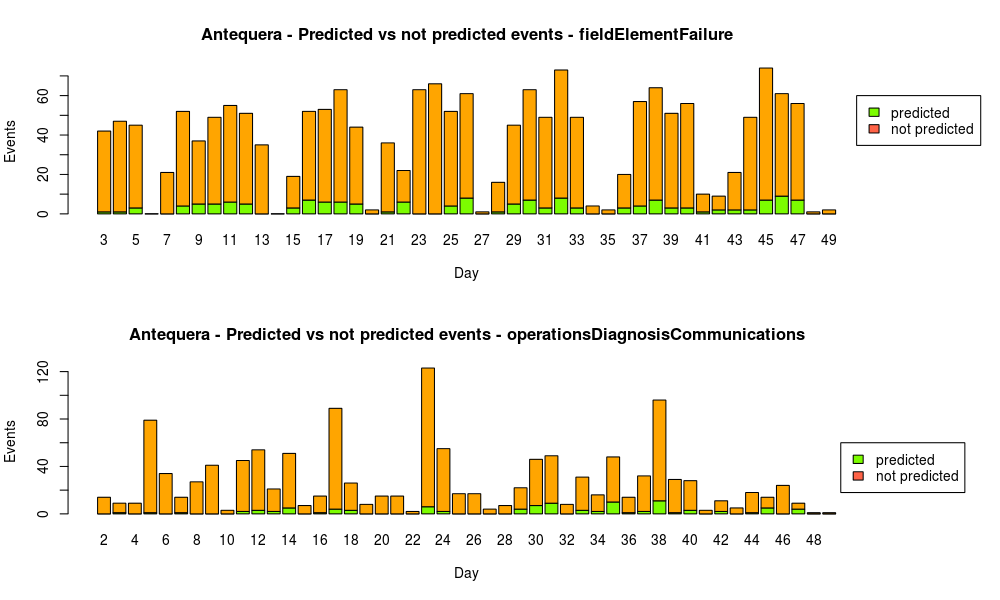
\includegraphics[width=\textwidth]{img/scenario_pred_notpred.png}
\caption{Timeline of predictions during a sample period} \label{fig:scenario_pred_notpred}
\end{figure}

\subsection{Percentage of right predictions}
To end with, we will analyse how many of the raised predictions are actually true. In order to illustrate better this aspect and take into account also the confidence parameter of the predictions, we will perform three different analysis: one disregarding predictions with $c < 0.5$, a second one with $c < 0.7$ and a third with $c < 0.8$. The results can be seen in figures \ref{fig:scenario_right_wrong}, \ref{fig:scenario_right_wrong_70} and \ref{fig:scenario_right_wrong_80} respectively.

As expected, when increasing the precision threshold we have less and less predictions, but these tend to be more accurate.

\begin{figure}[hbtp]
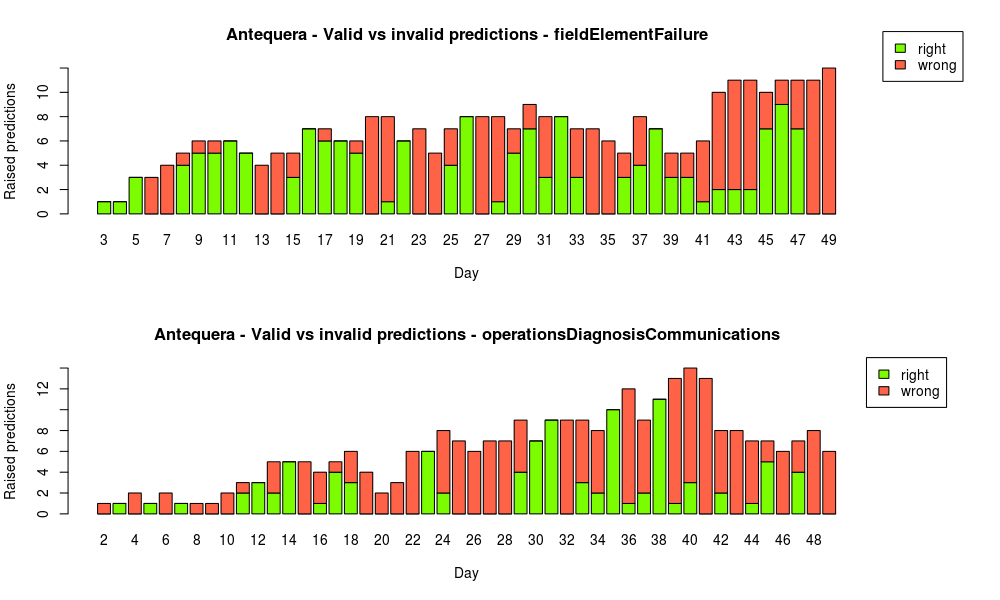
\includegraphics[width=\textwidth]{img/scenario_right_wrong.png}
\caption{Timeline of predictions during a sample period} \label{fig:scenario_right_wrong}
\end{figure}

\begin{figure}[hbtp]
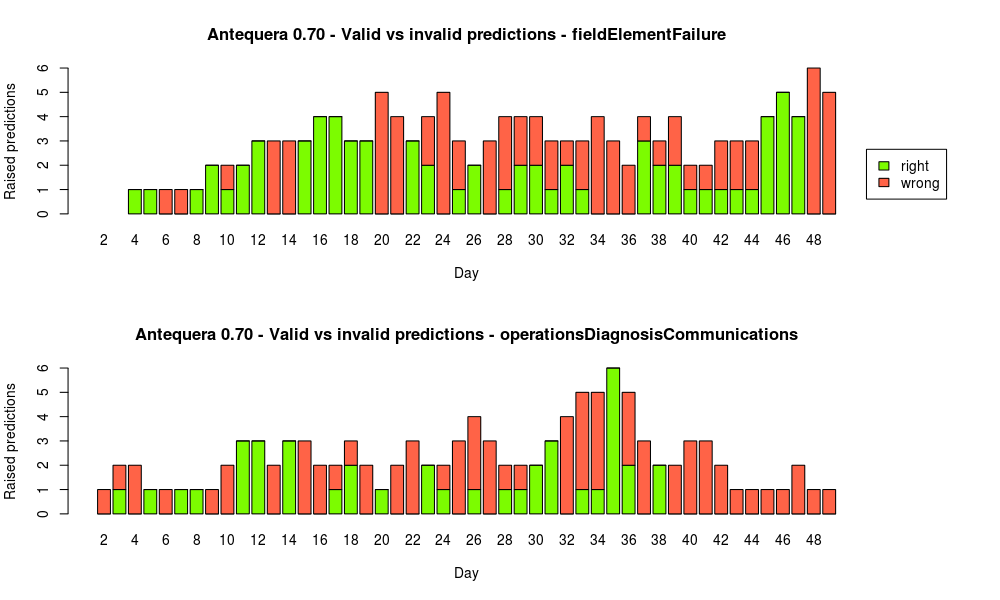
\includegraphics[width=\textwidth]{img/scenario_right_wrong_70.png}
\caption{Timeline of predictions during a sample period} \label{fig:scenario_right_wrong_70}
\end{figure}

\begin{figure}[hbtp]
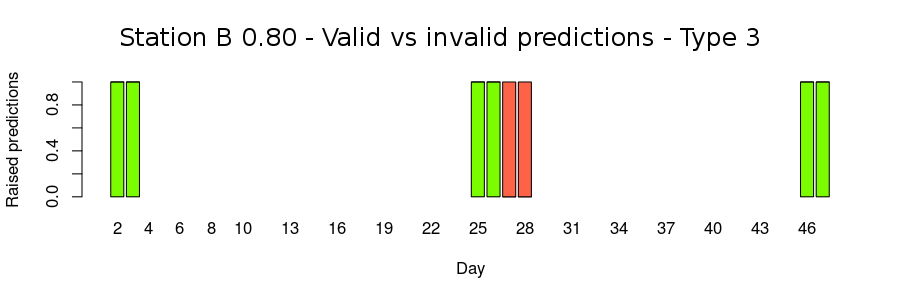
\includegraphics[width=\textwidth]{img/scenario_right_wrong_80.png}
\caption{Timeline of predictions during a sample period} \label{fig:scenario_right_wrong_80}
\end{figure}

\clearpage

\section{Conclusions}
The results obtained after the development of the presented procedures are found to be satisfactory, as shown in section~\ref{sec:desc_results}. Large rule sets with high precision values have been found for several stations and different time windows.

For this rulesets to be useful for Thales' operators, a implementation of a rule engine is necessary. This aspect with be covered in next stages of the project, and it is completely independent from the procedures described in this document which were used to obtain the predictive knowledge.

Also, results have been found to vary significantly in terms of quantity and precision in different stations and time periods, as seen in section~\ref{sec:desc_results}. In order to obtain higher quality results, it is necessary to explore alternative methods which can get over the limitations found with the performed method. First of all, the used algorithms can be vastly optimised to perform much better in our specific scenario. When searching for frequent sequences, we cannot limit the number of terms in the \emph{consequent}, as the maximum number of terms in each member of the sequence is fixed by a single parameter. In our case, we do not want to use sequences with more than one element in the consequent (as explained in section~\ref{sec:rule_model}) but our algorithm is still generating them as sequence candidates. This increases the complexity of the algorithm significantly, as we are growing our candidates in both the antecedent and the consequent of the rule while we only need the antecedent to grow.

Furthermore, as mentioned in section~\ref{sec:rule_model}, the candidates for rules are selected amongst sequences which are \emph{frequent}. Although this provides a good starting point in order to find predictive rules, we must perform two kinds of filtering in order to obtain the final rule sets: first by frequency, and later by precision. A new algorithm could be implemented in the same fashion as cSPADE, but performing only a filtering in terms of precision. This would not only save time and allow deeper searches, but also avoid disregarding those sequences which are not frequent but might lead to precise predictions.

Additionally, as seen in section~\ref{sec:datamining}, there are many other types of data mining algorithms which could be used or adapted to our problem. Specifically, a parallell approach has been made using \emph{Bayesian Networks}. These networks provide a very useful mathematical model which can be used to predict information in a similar fashion than the rules. However, it usually requires a deep previous knowledge on the events of the system and their possible relations in order to obtain their full potential. After building some of these models and obtaining said information from Thales' engineers, the model based on \emph{association rules} was still found to perform much better in all terms. Additional research would be necessary in order to obtain better results with these alternative tools.

Finally, we have found that one of the best and most immediate ways to increase the quality of the results is to divide the large datasets into smaller clusters. In section~\ref{sec:dataclustering} we have presented two possible clustering methods which have indeed improved the results significantly. Further improvement could be achieved by performing a deeper research on alternative clustering methods. Specifically, the method described in section~\ref{sec:group_elements} was found to increase peformance in very high rates. Developing a way to make this clustering method automatisable and directly feasible for all the stations would likely highly increase performance.

Summarising, in order to obtain higher quality results, a way must be found to face limits in terms of computation capabilities. The server available for our project is powerful enough as to think of improving hardware. Therefore, software and data optimisation is the only way to obtain significant improvement in the results.

\clearpage



\bibliographystyle{plain} 
\bibliography{datamining}

\end{document}


